\documentclass[11pt]{article}

\usepackage[T1]{fontenc}
\usepackage{lmodern}
\usepackage{amsmath,amssymb,amsthm}
\usepackage{graphicx}
\usepackage{array}
\usepackage{booktabs}
\usepackage[margin=1.1in]{geometry}
\usepackage[hidelinks]{hyperref}
\hypersetup{pdftitle={Minimal residual certificates for the
  Erdos-Straus conjecture: a verified census to 10\textasciicircum 12},
  pdfauthor={J. M. Hopkins}}
% Break URLs only at slashes, never inside hyphenated path components.
\def\UrlBreaks{\do\/}

\theoremstyle{plain}
\newtheorem{theorem}{Theorem}[section]
\newtheorem{proposition}[theorem]{Proposition}
\newtheorem{lemma}[theorem]{Lemma}
\newtheorem{corollary}[theorem]{Corollary}
\theoremstyle{remark}
\newtheorem{remark}[theorem]{Remark}
\theoremstyle{plain}
\newtheorem{hypothesis}[theorem]{Hypothesis}
\newtheorem{conjecture}[theorem]{Conjecture}

\numberwithin{equation}{section}
\emergencystretch=1.5em

\newcommand{\Hset}{\mathcal{H}}
\newcommand{\legendre}[2]{\genfrac{(}{)}{}{1}{#1}{#2}}
\DeclareMathOperator{\ord}{ord}

\title{Minimal residual certificates for the\\
Erd\H{o}s--Straus conjecture:\\
a verified census to $10^{12}$}

\author{J.~M.\ Hopkins\thanks{Independent researcher.
\texttt{jeff.m.hopkins@gmail.com}.
Computations and computer-assisted case analyses were carried out with the
code repository accompanying this paper:
\url{https://github.com/jeffmhopkins/Erd-s-Straus-attack}.}}

\date{August 2026}

\begin{document}
\maketitle

\begin{abstract}
The Erd\H{o}s--Straus conjecture asserts that $4/n = 1/a+1/b+1/c$ is
solvable in positive integers for every $n \ge 2$; the open cases
concentrate on primes in six residue classes mod $840$ (\emph{hard
primes}). Every solution at a hard prime $p$ has first denominator
$a = (p+R)/4$ for an \emph{admissible residual} $R \equiv 3 \pmod 4$,
and solvability at that $R$ is the divisor-class condition
$\exists\, k \mid m^2$, $m = pa$, with $k \equiv -m \pmod R$ --- a
criterion due to Bradford. The conjecture at $p$ is therefore exactly
the finiteness of the \emph{minimal working residual}
$R_{\min}(p)$, a structural invariant that verification records do
not report.

We compute and independently verify $R_{\min}$ for all
$1{,}175{,}215{,}396$ hard primes below $10^{12}$. The maximum is
$R_{\min} = 111$, first attained at $p = 119{,}945{,}383{,}009$; it
had stood at $107$ across the preceding five orders of magnitude,
and a heuristic model calibrated at $10^9$ predicted in advance both
the filling of a then-empty band $87 \le R \le 103$ and the decade
in which the record would move. Verification is graded: exhaustive
exact re-checking below $10^9$, complete deep tails and large
systematic samples above, every certificate re-verified as
$4abc = p(bc+ac+ab)$ in exact integer arithmetic, and all datasets
published with checksums.

Around the census we assemble the apparatus it exercises. There are
exact solvability criteria at $R = 3, 7, 11$ and at the first
composite residual $R = 15$; those at $R = 3, 7$ are Yamamoto's,
restated in residual form, while the exact criteria at $R = 11$ and
$R = 15$ are new. A support theorem --- the critical-number theorem
of Diderrich--Mann, transported to this setting --- shows that
failure at $R$ forbids at least half the unit classes mod $R$ on the
shifted form $(p+R)/4$, uniformly in $R$, and its classical
exceptions fall exactly at the residuals where an exact criterion is
available. The uniform consequence bounds $R_{\min}$ itself: all but
$O(x\exp(-c(\log\log x)^2))$ hard primes $p \le x$ satisfy
$R_{\min}(p) \le \varepsilon\log\log x$, with explicit certificates
--- a threshold exponentially smaller than the one implicit in
Vaughan's covering congruences at comparable exceptional-set
quality. The elementary layer and the finite enumerations behind the
criteria are machine-checked in Lean~4/\mbox{mathlib}.
\end{abstract}

\medskip
\noindent\textbf{2020 Mathematics Subject Classification.}
Primary 11D68; Secondary 11N35, 11Y50, 68V20.

\smallskip
\noindent\textbf{Keywords.} Erd\H{o}s--Straus conjecture, Egyptian
fractions, unit fractions, sieve methods, formal verification.

\section{Introduction}

Erd\H{o}s and Straus conjectured (see~\cite{Erdos50}) that for every
integer $n \ge 2$ the equation
\begin{equation}\label{eq:es}
  \frac{4}{n} \;=\; \frac{1}{a} + \frac{1}{b} + \frac{1}{c}
\end{equation}
has a solution in positive integers $a, b, c$. By multiplicativity it
suffices to treat prime $n$, and classical polynomial identities settle
every prime outside the six residue classes
\[
  \Hset \bmod 840 \;=\; \{1, 121, 169, 289, 361, 529\},
\]
the squares of units modulo $840$ (Mordell~\cite[Ch.~30]{Mordell}; the
quadratic-residue nature of the obstruction goes back to
Yamamoto~\cite{Yamamoto}). We call primes
in these classes \emph{hard primes}. Direct verification has confirmed the
conjecture far beyond any range considered here: to $10^{14}$ by Swett~\cite{Swett}, to $10^{17}$ by Salez~\cite{Salez}, and to $10^{18}$ by
Mihnea and Bogdan~\cite{MihneaBogdan}; the present paper is logically
independent of those bounds. The structure of
the solution count was analyzed by Elsholtz and Tao~\cite{ElsholtzTao}.
For calibration on the density axis: the first
density bounds on the exceptional set are due to Webb~\cite{Webb},
sieve bounds were advanced by Sander~\cite{Sander}, and
Vaughan's classical
mean-value bound~\cite{Vaughan} gives an exceptional set
$\ll x \exp(-c(\log x)^{2/3})$ for \eqref{eq:es} --- asymptotically
stronger than any fixed power of $\log x$, and still the record on
that axis.

This paper is about a different quantity, and it is primarily a
computation. A verification to $10^{18}$ answers ``is
\eqref{eq:es} solvable at $n$?'' and records a yes; it does not
record \emph{how hard} the instance was, and the published records do
not report the parameter in which the difficulty is measured. By
Proposition~\ref{prop:complete} --- Bradford's
criterion~\cite{Bradford}, restated --- every solution at a hard
prime $p$ is a certificate at some admissible residual
$R = 4a - p \equiv 3 \pmod 4$, and the conjecture at $p$ is exactly
the finiteness of the least such $R$, written $R_{\min}(p)$. Our
main object is a census of $R_{\min}$: its value for every one of the
$1{,}175{,}215{,}396$ hard primes below $10^{12}$, verified,
archived, and reproducible. What comes out of it is a distribution
with sharp structure (Section~\ref{sec:comp}), a broken record
(the maximum moves from $107$ to $111$ in the last decade computed),
and a heuristic model calibrated at $10^9$ whose advance predictions
about the tail were borne out at $10^{11}$ and $10^{12}$.

The rest of the paper is the apparatus the census exercises and the
structure it exhibits: exact per-residual solvability criteria
(Section~\ref{sec:exact}), which are what make the head of the
distribution computable in closed form; a support theorem valid at
every residual, which converts failure into a sieve condition; and,
as its capstone, an almost-all bound on $R_{\min}$ itself
(Theorem~\ref{thm:U}). Section~\ref{sec:context} states these and
sketches the sieve consequences; complete proofs of the elementary
layer, together with the finite enumerations behind the criteria,
are formalized in Lean~4 and inventoried in
Appendix~\ref{app:verif}.

\subsection*{New contributions}
\phantomsection\addcontentsline{toc}{subsection}{New contributions}

\paragraph*{The census.}
\begin{itemize}
\item $R_{\min}(p)$ computed and independently verified for every one
  of the $1{,}175{,}215{,}396$ hard primes $p < 10^{12}$
  (Section~\ref{sec:comp}), with the full distribution
  (Table~\ref{tab:dist}), a graded verification protocol
  (Appendix~\ref{app:verif}), and archived datasets carrying
  checksums.
\item The maximum of $R_{\min}$ moves for the first time in five
  orders of magnitude: it is $107$ throughout
  $10^7 \le x \le 10^{11}$ and $111$ at $10^{12}$, first attained at
  $p = 119{,}945{,}383{,}009$. Section~\ref{sec:comp} exhibits the
  certificate and the exhaustive refutation of every admissible
  $R \le 107$ at that prime.
\item A calibrated independence model, fitted to the complete $10^9$
  solvability masks, that predicted in advance both the population of
  the band $87 \le R_{\min} \le 103$ --- empty when the model was
  fitted --- and the decade in which the record would move. Both
  predictions were tested by the $10^{11}$ and $10^{12}$ runs and
  held (Section~\ref{sec:comp}).
\item A reproducibility layer: exact re-verification of every
  certificate as $4abc = p(bc+ac+ab)$, a Lean~4~\cite{Lean4} /
  \mbox{mathlib}~\cite{mathlib} formalization of the elementary layer
  and of the finite enumerations behind the exact criteria, and a
  published run kit. Appendix~\ref{app:verif} gives the inventory and
  the exact trust base.
\end{itemize}

\paragraph*{The apparatus, and what in it is new.}
\begin{itemize}
\item \emph{Exact} solvability criteria at $R = 11$
  (Theorem~\ref{thm:App}) and at the first composite residual
  $R = 15$ (Theorem~\ref{thm:R15}: a Jacobi-character dichotomy with
  no budget cases), together with the finite-reduction lemma
  (Theorem~\ref{thm:meta}) that licenses their enumeration. The
  criteria at $R = 3$ and $R = 7$ (Theorems~\ref{thm:A},
  \ref{thm:Ap}) are \emph{not} new --- they are Yamamoto's, in a
  different notation; see Remark~\ref{rem:yamamoto}, which also
  delimits what is new at $R = 11$ and $R = 15$.
\item A reciprocity identity (Theorem~\ref{thm:J}) collapsing the
  per-residual conditions into one global statement about $p$, which
  we use to describe the record prime mechanically.
\item The support theorem (Theorem~\ref{thm:S}): failure at $R$
  confines the factor classes of $(p+R)/4$ to at most half the unit
  classes mod $R$, for every admissible $R$ at once. As an additive
  statement this is the critical-number theorem of
  Diderrich--Mann~\cite{DiderrichMann}; the contribution here is the
  transport to residuals (bounded exponent budgets, a single
  prescribed target) and the observation that its classical
  exceptional groups occur exactly at $R = 3, 7, 15$, where
  Theorems~\ref{thm:A}, \ref{thm:Ap} and~\ref{thm:R15} supply an
  exact criterion --- so the sieve dimension $\tfrac12$ is available
  at every admissible residual with no gaps.
\item The sieve consequences (Section~\ref{sec:context}):
  certificate-producing exceptional-set bounds for every finite
  admissible list (Theorem~\ref{thm:FG},
  Proposition~\ref{prop:agg}, Theorem~\ref{thm:D}) and, as the
  capstone, the \emph{uniform chain} (Theorem~\ref{thm:U}): all but
  $O(x e^{-c(\log\log x)^2})$ hard primes $p \le x$ have
  $R_{\min}(p) \le \varepsilon\log\log x$, with an explicit
  certificate for each. Remark~\ref{rem:vaughan} states precisely
  what this does and does not improve on.
\item An open problem carved out of the ceiling of that argument:
  Conjecture~\ref{conj:A}, an aperiodic branch-classification
  statement, verified exhaustively in the accessible range, whose
  resolution would raise the bound to
  $R_{\min}(p) \le (\log x)^{c_0}$ (Theorem~\ref{thm:Upay}).
\end{itemize}

Read as a whole, the paper has three layers. \textup{(1)}~An exact
reformulation of solvability --- every solution of \eqref{eq:es} at a
hard prime is a residual certificate
(Proposition~\ref{prop:complete}), which is Bradford's criterion.
\textup{(2)}~Finite, machine-checkable inputs at individual
residuals: the exact criteria (Theorems~\ref{thm:A}--\ref{thm:R15}),
the reciprocity identity (Theorem~\ref{thm:J}), and the support
bounds (Lemma~\ref{lem:S}, Theorem~\ref{thm:S}). \textup{(3)}~The
census of Section~\ref{sec:comp}, which is what layers (1)--(2) are
for: they make $R_{\min}$ computable at scale, and the exact criteria
determine the head of its distribution in closed form. The sieve
consequences of Section~\ref{sec:context} run in the other
direction, predicting the shape of the tail; the computation
calibrates them and tests what they predict.

\subsection{The residual method}\label{sec:intro-method}

Fix a hard prime $p$. All six classes satisfy
\[
  \text{(H1) } p \equiv 1 \pmod 8, \qquad
  \text{(H2) } p \equiv 1 \pmod 3, \qquad
  \text{(H3) } p \bmod 7 \in \{1, 2, 4\}.
\]
For an \emph{admissible residual} $R \equiv 3 \pmod 4$ put
\[
  a \;=\; \frac{p+R}{4} \in \mathbb{Z}, \qquad m \;=\; pa.
\]
Substituting $a$ into \eqref{eq:es} and clearing denominators shows that a
solution with first denominator $a$ exists if and only if
\begin{equation}\label{eq:cert}
  \exists\, k \mid m^2 \quad\text{with}\quad k \equiv -m \pmod R,
\end{equation}
in which case $b = (k+m)/R$ and $c = (m^2/k + m)/R$ are positive integers
solving \eqref{eq:es}. We write $R_{\min}(p)$ for the least admissible $R$
for which \eqref{eq:cert} holds. The formulation loses no solutions:

\begin{proposition}[completeness]\label{prop:complete}
Every solution of \eqref{eq:es} at a hard prime $p$, ordered
$a \le b \le c$, has $p/4 < a \le 3p/4$; hence $R = 4a - p$ is an
admissible residual in $(0, 2p]$ and the solution is a residual
certificate at $R$. Consequently $R_{\min}(p) \le 2p$ if and only if
the conjecture holds at $p$.
\end{proposition}

\begin{proof}
With $a \le b \le c$, the equation gives $1/a < 4/p \le 3/a$, so
$p/4 < a \le 3p/4$ and $R = 4a - p \in (0, 2p]$; $R \equiv 3 \pmod 4$
is automatic from $p \equiv 1 \pmod 4$. By the displayed equivalence,
the solution yields a divisor $k$ as in \eqref{eq:cert}, so
$R_{\min}(p) \le R \le 2p$. Conversely \eqref{eq:cert} at any
admissible $R$ produces a solution.
\end{proof}

A word on provenance. Proposition~\ref{prop:complete} is not new.
The bounded search space together with the divisor-congruence
criterion modulo $4a - p$ is due to Bradford~\cite{Bradford}, who
proves that a solution exists at $p$ if and only if some $a$ in
$\lceil p/4 \rceil \le a \le \lceil p/2 \rceil$ admits a divisor of
$a^2$ in a prescribed class modulo $4a - p$ --- his range is in fact
slightly sharper than the $a \le 3p/4$ recorded above, and the
correspondence with solutions is likewise bijective. These are by now
called the Bradford conditions~\cite{MihneaBogdan}. Criteria of this
general shape go back further. Yamamoto~\cite{Yamamoto} constructs a
complete system $\Sigma$ of solvable coverings and proves that
$4/p$ is solvable if and only if $p$ lies in their union; his
simplified subsystem $\Sigma_0$ is defined on precisely the six hard
classes, and the individual coverings $\{-s/q\} = \{n : q \mid n+s\}$
are, for odd $q$, exactly the condition ``$q$ divides
$(p+s)/4$''. So Yamamoto's system is a residual-indexed criterion in
different notation, and several of the per-residual statements below
are his; Remark~\ref{rem:yamamoto} makes the dictionary explicit and
says which are. Lopez~\cite{Lopez} states the same shift-indexed
divisor condition in general form for one solution shape. Mordell's
Chapter~30~\cite[Ch.~30]{Mordell} collects the classical identities
and his own non-existence theorem; the systematic divisor-counting
form is Elsholtz--Tao's~\cite{ElsholtzTao}; and
Salez~\cite{Salez} proves a completeness theorem for seven modular
equations at the level of degree-one prime polynomials.

What this paper does with the criterion is to \emph{measure} it. The
organizing move is to index by the residual $R$ rather than by the
denominator $a$, which makes $R_{\min}(p)$ a well-defined statistic
of $p$ and the object of a census: it is computable at scale because
each fixed $R$ admits a finite exact criterion
(Theorem~\ref{thm:meta}), determined in closed form at
$R = 3, 7, 11, 15$, and because failure at every other $R$ is
constrained uniformly (Theorem~\ref{thm:S}). Bradford's range gives
$R_{\min}(p) \ll p$; the computation of Section~\ref{sec:comp}
shows $R_{\min} \le 111$ throughout $p < 10^{12}$, and
Theorem~\ref{thm:U} bounds it by $\varepsilon\log\log x$ for almost
every hard prime.

Two
elementary congruences drive everything below. From $4a = p + R$,
\begin{equation}\label{eq:star}
  a \equiv 4^{-1}p, \qquad m \equiv 4^{-1}p^2 \pmod R,
\end{equation}
and since $\gcd(p, R) = 1$ (as $p$ is prime and $R \ne p$,
$R \equiv 3 \not\equiv p \pmod 4$), also
$\gcd(a, R) = \gcd(m, R) = 1$: the setting is always a unit computation
modulo $R$. By \eqref{eq:star}, $m$ is a \emph{square} modulo every prime
$r \mid R$; hence for every prime $r \mid R$ with $r \equiv 3 \pmod 4$
(at least one exists, since $R \equiv 3 \pmod 4$),
\begin{equation}\label{eq:target}
  \legendre{-m}{r} \;=\; \legendre{-1}{r}
  \;=\; -1
\end{equation}
--- \emph{the target class $-m$ is a quadratic non-residue mod $r$.}

\paragraph{A worked example.} Take the hard prime $p = 1009$
($\equiv 169 \pmod{840}$) and the smallest admissible residual $R = 3$.
Then $a = (1009+3)/4 = 253 = 11 \cdot 23$ and $m = pa = 255{,}277$.
Since $11 \equiv 2 \pmod 3$, Theorem~\ref{thm:A} below promises a
certificate: take $k = 11$, a divisor of $m^2$ with
$k \equiv -m \equiv 2 \pmod 3$. Then $b = (k+m)/3 = 85{,}096$ and
$c = (m^2/k+m)/3 = 1{,}974{,}822{,}872$, and indeed
\[
  \frac{4}{1009} \;=\; \frac{1}{253} + \frac{1}{85{,}096}
  + \frac{1}{1{,}974{,}822{,}872}.
\]
Had every prime factor of $a$ been $\equiv 1 \pmod 3$, every divisor of
$m^2$ would be $\equiv 1 \pmod 3$ and the required class $2$ would be
unreachable --- the prototype of all the obstructions studied below.

\paragraph{The shape of what follows.} Everything in this paper grows
out of the picture just seen, read at three levels. \emph{Locally}
(one residual): whether the target class $-m$ is attainable from the
factor classes of $a$ is a question about a finite multiplicative
state --- the multiset of classes with bounded exponent budgets --- so
each fixed $R$ admits an exact, machine-enumerable solvability
criterion (Theorems~\ref{thm:A}--\ref{thm:App} below). This is what
makes the census of Section~\ref{sec:comp} feasible: the head of the
distribution of $R_{\min}$ is decided by a character test rather
than a divisor search. \emph{Globally} (all residuals at once): the
conditions entering these
criteria are quadratic characters, and reciprocity folds the condition
at every residual into signs $\legendre{p}{q}$ indexed by the primes
$q$ dividing the shifted values $(p+R)/4$ --- failures at different
residuals correlate because shifted values share prime factors
(Theorem~\ref{thm:J}). \emph{Quantitatively}: each criterion says that
failure forces $(p+R)/4$ to avoid prime factors in many residue
classes, a sifting condition; stacking residuals multiplies the
savings (Theorem~\ref{thm:FG}), though it provably cannot reach
emptiness (Remark~\ref{rem:emptiness}) --- the honest endpoint of the
method, discussed in Section~\ref{sec:open}.

\subsection{Main results}

\begin{theorem}[$R=3$; exact]\label{thm:A}
Let $p \equiv 1 \pmod 4$ be prime with $3 \nmid p$, and $a = (p+3)/4$. Then
\eqref{eq:cert} holds for $R = 3$ if and only if $a$ has a prime factor
$q \equiv 2 \pmod 3$. When it does, $k = q$ is a certificate.
\end{theorem}

Modulo $3$, character equals class and the criterion is elementary.
For every other fixed residual we need to know that the search space
is finite before we can enumerate it, which is the content of the
next statement. We label it a theorem for reference, but it is
bookkeeping on top of Bradford's criterion, and finite-generation
statements of this kind have a long history in the subject:
Terzi~\cite{Terzi} generated $198$ solvable residue classes modulo
$120120$ algorithmically, Yamamoto's~\cite[\S3]{Yamamoto} whole
apparatus is a finite generation procedure for solvable coverings,
and Salez~\cite{Salez} proves a completeness theorem for polynomial
families. What is specific here is the finite datum: the capped
multiset of factor classes of $(p+R)/4$ together with $p \bmod R$.

\begin{theorem}[finite reduction]\label{thm:meta}
For every fixed prime $R \equiv 3 \pmod 4$, the validity of
\eqref{eq:cert} at a hard prime $p$ depends only on \textup{(i)} the
multiset of classes mod $R$ of the prime factors of $a = (p+R)/4$, with
multiplicities capped at $\lceil (R-1)/2 \rceil$, and \textup{(ii)}
$p \bmod R$. Consequently an exact solvability criterion exists for every
$R$ and is computable by finite enumeration.
\end{theorem}

\begin{theorem}[$R=7$, hard primes; exact]\label{thm:Ap}
Let $p$ be a hard prime and $a = (p+7)/4$. Then \eqref{eq:cert} holds for
$R = 7$ if and only if $a$ has a prime factor that is a quadratic
non-residue modulo $7$.
\end{theorem}

\begin{theorem}[$R=11$, hard primes; exact]\label{thm:App}
Let $p$ be a hard prime and $a = (p+11)/4$; note $3 \mid a$, $2 \nmid a$,
$7 \nmid a$ automatically. Then \eqref{eq:cert} \emph{fails} for $R = 11$
if and only if either
\begin{itemize}
\item[(a)] every prime factor of $a$ is a quadratic residue mod $11$; or
\item[(b)] $v_3(a) = 1$, every other prime factor of $a$ is
  $\equiv 1 \pmod{11}$ except a \emph{non-residue part} --- its factors
  in the non-residue classes mod $11$ --- of exactly one of the
  shapes
  \[
    \{q \equiv 2\}, \qquad \{q \equiv 6\}, \qquad
    \{q \equiv 2\} \cup \{q' \equiv 6\} \pmod{11},
  \]
  each with multiplicity one, paired respectively with
  $p \equiv 2,\ 6,\ 1 \pmod{11}$.
\end{itemize}
\end{theorem}

For composite $R$ the certificate condition couples the prime-power
components of $R$ through the Chinese Remainder Theorem, and the
divisor-class computation lives in the (generally non-cyclic) unit
group $(\mathbb{Z}/R)^*$. Theorem~\ref{thm:meta} holds verbatim with
$(\mathbb{Z}/R)^*$ in place of the cyclic group (multiplicities capped
once exponent ranges cover each class's cyclic span; see
Remark~\ref{rem:cap}). The first composite case turns out to be
\emph{simpler} than $R = 11$: a pure character dichotomy, with the
quadratic character modulo a prime replaced by the Jacobi character
modulo $15$, and no budget cases at all.

\begin{theorem}[$R=15$, hard primes; exact]\label{thm:R15}
Let $p$ be a hard prime and $a = (p+15)/4$; note $p \bmod 15 \in
\{1, 4\}$ and $2 \mid a$ automatically. Then \eqref{eq:cert} holds for
$R = 15$ if and only if $a$ has a prime factor $q$ with
$\legendre{q}{15} = -1$, i.e.\ $q \equiv 7, 11, 13, 14 \pmod{15}$.
\end{theorem}

\begin{remark}[attribution at $R = 3, 7, 11, 15$]\label{rem:yamamoto}
Theorems~\ref{thm:A} and~\ref{thm:Ap} are not new. In
Yamamoto's notation~\cite[\S3]{Yamamoto} the covering
$\{-s/q\}$ --- the set of $n$ with $q \mid n+s$, equivalently, for
odd $q$, $q \mid (n+s)/4$ --- lies in his system $\Sigma_1$ of
solvable coverings exactly for
$q \equiv -1 \pmod 3$ when $s = 3$, and for
$q \equiv -1, -2, -4 \pmod 7$ when $s = 7$; he records the
common form explicitly, noting that ``all the coverings $\{-s/q\}$
with the Jacobi symbol $\smash{\legendre{-s}{q}} = -1$ are contained
in $\Sigma_1$, for $s = 1, 2, 3, 4, 7$ and $8$''
\cite[p.~45]{Yamamoto}, and $\Sigma_1$ is defined on precisely the
six hard classes. Since $\smash{\legendre{-s}{q}} =
\smash{\legendre{q}{s}}$ for $s \equiv 3 \pmod 4$, and since
membership of a non-residue class is inherited by some prime factor,
this is the sufficiency half of Theorems~\ref{thm:A} and~\ref{thm:Ap}
verbatim; the necessity half is the character obstruction
(Proposition~\ref{prop:char}), which is Yamamoto's Lemma~4
specialised. What the statements below add at these two residuals is
only that the certificate can be taken at residual exactly $R$, and
a machine-checked proof.

At $R = 11$ and $R = 15$ the situation is different, and it is worth
being exact about the boundary. Yamamoto's Table~3
\cite[p.~45]{Yamamoto} gives, for $s = 11$, the classes
$q \equiv -1, -3, -4 \equiv 7, 8, 10 \pmod{11}$: precisely the three
non-residue classes in which a single prime factor already forces
solvability. Theorem~\ref{thm:App} supplies the complement --- that
$q \equiv 2$ and $q \equiv 6 \pmod{11}$ suffice as well, outside the
explicitly described budget family of case~(b) --- and the exactness.
Over the $1{,}005$ hard primes below $4 \times 10^5$, Yamamoto's
classes certify $413$ and Theorem~\ref{thm:App} certifies $628$.
Yamamoto does not treat $s = 15$ (his tables list prime $s$ only),
but his constructions (i)--(ii) apply verbatim there and yield the
three classes $q \equiv 7, 13, 14 \pmod{15}$;
Theorem~\ref{thm:R15} completes the Jacobi dichotomy with the fourth
class $q \equiv 11 \pmod{15}$ and proves it exact ($315$ versus
$355$ primes certified in the same range). For $R \ge 19$ the
divergence is no longer marginal: Yamamoto's rules give $1$, $3$ or
$9$ classes according to $R \bmod 24$, against the $(R-1)/2$
non-residue classes reached by the criteria and support bounds
below --- $3$ versus $53$ at $R = 107$.
\end{remark}

\begin{remark}[computer-assisted components]\label{rem:computer}
The exhaustive verifications behind Theorems~\ref{thm:Ap},
\ref{thm:App}, \ref{thm:R15} and Lemma~\ref{lem:S} below are \emph{parts of the
respective proofs}, on the same footing as a hand case analysis. Each is
a deterministic enumeration of a finite configuration space whose
finiteness and sufficiency are proved in advance
(Theorem~\ref{thm:meta}; for Lemma~\ref{lem:S}, monotonicity of
target-reachability in support and multiplicities, checked at minimal
exponents). The checks are short (seconds each, up to $331$\,s for the largest,
$R = 107$), involve only exact integer arithmetic, and the code is
available in the
accompanying repository; Table~\ref{tab:components} records the exact
configuration counts and entry points. The enumerations at
$R = 7, 11$ and the $R = 19, 23, 31$ cases of Lemma~\ref{lem:S} are
additionally formalized in Lean~4, with the reductions they rely on
proved as theorems rather than trusted (the $R = 15$ enumeration and
the remaining cases of Lemma~\ref{lem:S} run in the Python layer
only); Appendix~\ref{app:verif} gives the inventory and the exact
trust base.
\end{remark}

The obstruction framework of Section~\ref{sec:obstruction} yields a
reciprocity identity that converts the per-residual conditions into a
single global statement about $p$ --- a structural interpretation of
joint failure across residuals:

\begin{theorem}[reciprocity structure]\label{thm:J}
Let $p$ be a hard prime, $R \equiv 3 \pmod 4$ prime, and $q$ an odd
prime factor of $a = (p+R)/4$ (necessarily $q \ne R$). Then
\[
  \legendre{q}{R} \;=\; \legendre{p}{q}.
\]
\end{theorem}

The sieve consequences below need one input per residual: a statement
that failure at $R$ forces the shifted form $(p+R)/4$ to avoid prime
factors in a positive-density set of residue classes. For
$R = 3, 7, 11, 15$ the exact criteria provide this; for every other
residual it is the support bound, which we state first in the
per-residual machine-verified form in which it was originally
established (Lemma~\ref{lem:S}) and then prove unconditionally for
every residual at once (Theorem~\ref{thm:S}; both proved in
Section~\ref{sec:sieve}).

\begin{lemma}[support bound; verified for every prime
$R \equiv 3 \pmod 4$, $19 \le R \le 107$]\label{lem:S}
Let $R$ be one of the twelve primes
$19, 23, 31, 43, 47, 59, 67, 71, 79, 83, 103, 107$, and call the set of
unit classes mod $R$ occupied by the prime factors of $(p+R)/4$ its
\emph{support}. Every configuration for which residual $R$ fails at a
hard prime has support of size at most $(R-1)/2$, at most $(R-3)/2$ of
whose classes differ from the identity class (which never affects
solvability). Consequently failure at $R$ forbids at least half the
classes, through finitely many maximal-support branches.
\end{lemma}

\begin{theorem}[unconditional support bound]\label{thm:S}
\textup{(i)} Let $d \ge 4$ be even and $S \subseteq \mathbb{Z}/d
\setminus \{0\}$. If the bounded subset-sum set
\[
  M(S) \;=\; \Bigl\{ \textstyle\sum_{v \in S} e_v v \;:\;
  e_v \in \{0, 1, 2\} \Bigr\}
\]
is not all of $\mathbb{Z}/d$, then $|S| \le d/2 - 1$, and the bound is
attained ($S =$ the nonzero even classes). \textup{(ii)} Consequently,
for \emph{every} prime $R \equiv 3 \pmod 4$ and every $p$: if the prime
factors of $(p+R)/4$ occupy at least $(R-1)/2$ nonzero unit classes
mod $R$, then every unit class is a divisor class of $m^2$ and
\eqref{eq:cert} holds; failure forces the conclusion of
Lemma~\ref{lem:S}, with no upper limit on $R$. \textup{(iii)} In a
finite abelian group $G$ of even order $g$ with $t$ involutions
(multiplicative form, $M(S) = \prod_{v \in S}\{1, v, v^2\}$): if
$M(S) \ne G$ then $|S| \le \max(\lfloor (g+t-2)/2 \rfloor,\, g/2 - 1)$.
For $G = (\mathbb{Z}/R)^*$ with $\omega(R) \le 2$ this is $\le g/2$, so
failure at any admissible composite $R$ forbids at least
$\varphi(R)/2 - 1$ unit classes on $(p+R)/4$ --- sieve dimension
$\ge \tfrac12 - 1/\varphi(R)$. For the admissible composites
$R \le 107$ an exhaustive enumeration
(\texttt{kneser\_support\_general}, a proof component of this clause)
sharpens the maximal failing support to $g/2 - 1$, so those residuals
forbid at least $\varphi(R)/2$ classes and join the chain with full
dimension $\ge \tfrac12$ each. For arbitrary $\omega(R)$ the same
bound reads $|S| \le \max(\lfloor (g+t-2)/2 \rfloor,\, g/2 - 1)$ with
$t = 2^{\omega(R)} - 1$, so failure forbids at least
$(g-t)/2 - 1 \ge \varphi(R)/2 - 2^{\omega(R)-1} - 1$ unit classes ---
dimension $\ge \tfrac12 - (2^{\omega(R)-1}+1)/\varphi(R)$, and since
$2^{\omega(R)} = R^{o(1)}$ this is $\ge 0.44$ for every admissible
$R$ beyond an absolute bound: \emph{every} residual, with no
restriction on $\omega$, is a usable sieve input.
\end{theorem}

\begin{theorem}[the chain]\label{thm:FG}
The number of hard primes $p \le x$ failing every residual in
$\{3, 7\}$, in $\{3, 7, 11\}$, in $\{3, 7, 11, 15\}$, and in
$\{3, 7, 11, 15, 19\}$ is, respectively,
\[
  O\!\left(\frac{x}{(\log x)^{2}}\right), \qquad
  O\!\left(\frac{x}{(\log x)^{5/2}}\right), \qquad
  O\!\left(\frac{x}{(\log x)^{3}}\right), \qquad
  O\!\left(\frac{x}{(\log x)^{7/2}}\right).
\]
More generally, by Theorem~\ref{thm:S}, for \emph{every} finite set
$\mathcal{P}$ of admissible residuals $R \equiv 3 \pmod 4$ --- prime,
or composite with $\omega(R) \le 2$ --- the number of hard primes
failing every residual in $\mathcal{P}$ is
$O_{\mathcal{P}}\!\left(x/(\log x)^{1+\kappa(\mathcal{P})}\right)$,
where $\kappa(\mathcal{P}) = \sum_{R \in \mathcal{P}} \delta_R$ with
$\delta_R = \tfrac12$ for $R$ prime or composite $\le 107$ and
$\delta_R = \tfrac12 - 1/\varphi(R)$ for composite $R > 107$
(the two tiers of Theorem~\ref{thm:S}(iii)); in particular
$\kappa(\mathcal{P}) = |\mathcal{P}|/2$ for every list drawn from the
residuals up to $107$. For the fifteen primes $\equiv 3 \pmod 4$ up to
$107$ the exponent is $17/2$, and for the full $27$-element admissible
list $\{3, 7, 11, \dots, 107\}$ it is $29/2$. All but a proportion
$O((\log x)^{-2})$ of hard primes are solved within
$\{3, 7, 11, 15\}$ --- one power of $\log x$ less than the counts
above, since there are $\asymp x/\log x$ hard primes up to $x$.
\end{theorem}

\begin{proposition}[aggregate identity families]\label{prop:agg}
Let $p \equiv 1 \pmod 4$ be prime and $R \equiv 3 \pmod 4$. If
$R \mid p+1$, then $k = a p^2$ is a certificate for residual $R$; if
$R \mid p+4$, then $k = a^2 p$ is. Hence any prime factor
$\equiv 3 \pmod 4$ of $p+1$ or of $p+4$ yields an explicit solution,
and no divisor shape $k = a^j p^i$ yields a further $p$-only
condition. Adding the two corresponding linear forms to
Theorem~\ref{thm:FG}: the number of hard primes $p \le x$ failing every
prime residual up to $107$ and both families is
$O(x/(\log x)^{19/2})$; with the full $27$-element admissible list the
exponent is $31/2$.
\end{proposition}

\begin{theorem}[density reduction]\label{thm:D}
For every $A > 0$ there is a finite admissible set $S(A)$ such that the
number of hard primes $p \le x$ for which every residual in $S(A)$ fails
is $O_A\!\left(x/(\log x)^{1+A}\right)$.
\end{theorem}

\begin{remark}[relation to Vaughan's bound]\label{rem:vaughan}
As exceptional-set estimates, Theorem~\ref{thm:D}, the chain of
Theorem~\ref{thm:FG}, and Theorem~\ref{thm:U} are all weaker than
Vaughan's bound
$\ll x \exp(-c(\log x)^{2/3})$~\cite{Vaughan}, which already exceeds
every fixed power of $\log x$. They are not offered as improvements
on it, and the honest comparison needs one further step, because
Vaughan's argument is \emph{constructive}: it proceeds by covering
congruences, and every $n$ it certifies comes with an explicit
solution and hence with an explicit admissible residual, bounded by
a power of his sifting parameter. Read that way it already gives an
almost-all bound on $R_{\min}$ --- roughly
$R_{\min}(n) \le \exp(O((\log x)^{1/3}))$ outside a set of size
$x\exp(-c(\log x)^{2/3})$, and $R_{\min}(n) \le (\log x)^{\theta}$
outside $x\exp(-c(\log\log x)^2)$ when the threshold is set to match
Theorem~\ref{thm:U}'s exceptional set. So Theorem~\ref{thm:U} is not
the first almost-all bound on $R_{\min}$. Its content is that at
comparable exceptional-set quality it lowers the threshold from a
power of $\log x$ to a constant multiple of $\log\log x$ --- an
exponential gain in the certified residual, which is the quantity
Proposition~\ref{prop:complete} shows \emph{is} the conjecture at
$p$. Two further differences of kind: the exceptional sets here are
cut out by finitely many \emph{explicit} multiplicative conditions on
shifted forms, each failure constructively certified by an exhibited
divisor $k$, with the underlying lemmas exact or machine-verified;
and the certificates are of a single controlled shape, indexed by
$R$, rather than assembled from a covering system. A mean-value
argument, by contrast, counts the primes that fail and produces no
residual at all for the ones that succeed.
\end{remark}

\emph{Organization.}
Section~\ref{sec:obstruction} develops the obstruction framework
(Propositions~\ref{prop:char}, \ref{prop:succ}) and proves
Theorem~\ref{thm:J}, whose Corollary~\ref{cor:J} depends on the
character/II dichotomy introduced there.
Section~\ref{sec:exact} proves Theorem~\ref{thm:A}, then
Theorem~\ref{thm:meta}, then Theorems~\ref{thm:Ap}, \ref{thm:App}
and~\ref{thm:R15}, which rest on it. Section~\ref{sec:comp} is the
census: data, verification protocol, the record, and the calibrated
model. Section~\ref{sec:context} is the structural context ---
Section~\ref{sec:sieve} proves
Theorem~\ref{thm:FG} (base case first, then, after the monotonicity
reduction (Lemma~\ref{lem:mono}), Lemma~\ref{lem:S} and its
unconditional upgrade Theorem~\ref{thm:S}, the higher
exponents), followed by Proposition~\ref{prop:agg} and
Theorem~\ref{thm:D}; Section~\ref{sec:uniform} proves the uniform
chain (Theorem~\ref{thm:U}); Section~\ref{sec:branch} localizes
what stands between it and a polylogarithmic bound; and
Section~\ref{sec:ladder} sketches, in compressed form, the one
conditional program that would pass the ceiling.

Table~\ref{tab:deps} records, for each main result, exactly what its
proof consumes and its formal-verification status, so that each layer
can be audited independently.

\begin{table}[ht]
\centering
\small
\begin{tabular}{>{\raggedright\arraybackslash}p{2.6cm}>{\raggedright\arraybackslash}p{5.3cm}l>{\raggedright\arraybackslash}p{3.6cm}}
\toprule
result & proof inputs & proved in & machine-checked? \\ \midrule
Prop.~\ref{prop:complete} & elementary & \S\ref{sec:intro-method} & Lean, both directions \\ \addlinespace
Props.~\ref{prop:char}, \ref{prop:succ} & elementary (characters; explicit $k$) & \S\ref{sec:obstruction} & Lean \\ \addlinespace
Thm.~\ref{thm:A} ($R{=}3$) & elementary & \S\ref{sec:exact} & Lean, both directions \\ \addlinespace
Thm.~\ref{thm:meta} & elementary & \S\ref{sec:exact} & model + reduction in Lean \\ \addlinespace
Thm.~\ref{thm:Ap} ($R{=}7$) & Prop.~\ref{prop:char} + Thm.~\ref{thm:meta} + enumeration ($1{,}536$) & \S\ref{sec:exact} & Lean (\texttt{native\_decide}) \\ \addlinespace
Thm.~\ref{thm:App} ($R{=}11$) & Thm.~\ref{thm:meta} + enumeration ($497{,}664$) & \S\ref{sec:exact} & Lean (\texttt{native\_decide}) \\ \addlinespace
Thm.~\ref{thm:R15} ($R{=}15$) & Thm.~\ref{thm:meta}, composite form + enumeration ($349{,}920$) & \S\ref{sec:exact} & Lean (\texttt{native\_decide}) \\ \addlinespace
Thm.~\ref{thm:J} & quadratic reciprocity & \S\ref{sec:obstruction} & Lean \\ \addlinespace
Lem.~\ref{lem:S} & Lem.~\ref{lem:mono} + enumerations / DP & \S\ref{sec:sieve} & Lean at $R = 19, 23, 31$ \\ \addlinespace
Thm.~\ref{thm:S} & Kneser's theorem + Lem.~\ref{lem:mono}; (iii) upgrade at $R \le 107$: enumeration & \S\ref{sec:sieve} & Lean, parts (i) and (iii); (iii) upgrade: Python \\ \addlinespace
Thm.~\ref{thm:FG} & Thms.~\ref{thm:A}, \ref{thm:Ap}--\ref{thm:R15}, \ref{thm:S} + Fundamental Lemma & \S\ref{sec:sieve} & no \\ \addlinespace
Prop.~\ref{prop:agg} & elementary + Thm.~\ref{thm:FG} & \S\ref{sec:sieve} & families in Lean \\ \addlinespace
Thm.~\ref{thm:D} & Prop.~\ref{prop:succ} + Fundamental Lemma & \S\ref{sec:sieve} & no \\ \addlinespace
Thm.~\ref{thm:U} & Thm.~\ref{thm:S}(iii), general tier + Brun's sieve, uniform constants & \S\ref{sec:sieve} & no \\ \addlinespace
Thm.~\ref{thm:Mcount} & explicit construction (complete partitions) & \S\ref{sec:sieve} & Lean \\ \addlinespace
Thm.~\ref{thm:Mkernel} & Kneser + Lem.~\ref{lem:mono} + quotient induction & \S\ref{sec:sieve} & Lean, single step \\ \addlinespace
Thm.~\ref{thm:Mcont} & Thm.~\ref{thm:Mkernel} + Conjecture~\ref{conj:A} & \S\ref{sec:sieve} & no (conditional) \\ \addlinespace
Prop.~\ref{prop:betavac} & elementary (isolation of punctures) & \S\ref{sec:sieve} & Lean \\ \addlinespace
Thm.~\ref{thm:Upay} & Thm.~\ref{thm:Mcont} + the audit of Thm.~\ref{thm:U} & \S\ref{sec:sieve} & no (conditional) \\ \addlinespace
Lems.~\ref{lem:Jcomp}--\ref{lem:N} & Jacobi reciprocity, elementary & \S\ref{sec:ladder} & Lean \\ \addlinespace
Thms.~\ref{thm:L0}, \ref{thm:B1} & Thm.~\ref{thm:S} / Prop.~\ref{prop:succ} + sieve & \S\ref{sec:ladder} & no \\ \addlinespace
Thm.~\ref{thm:sharp} & norm-form bridge \eqref{eq:normform} + \cite{IwaniecPhiA}, \cite{FHRSS} + Fundamental Lemma & \S\ref{sec:ladder} & no \\ \addlinespace
Thm.~\ref{thm:L1} & Hypothesis~\ref{hyp:B} (measured) + large sieve & \S\ref{sec:ladder} & no (conditional) \\
\bottomrule
\end{tabular}
\caption{Audit map: what each main result depends on, where it is
proved, and its formal-verification status. ``---'' means the result
is elementary enough that no machine check was warranted; ``no'' means
the proof is by hand only. Theorem~\ref{thm:sharp} is established in
outline (proof sketch).}
\label{tab:deps}
\end{table}

Three printed results are retained as stepping stones although later
results subsume them, and the reader may want the map stated once:
Theorem~\ref{thm:D} is superseded by Theorem~\ref{thm:U} (which gives
$(\log x)^{-A}$ for every $A$ at once), but its fixed-list proof is
simpler and is the template the uniform chain scales; Lemma~\ref{lem:S}
is subsumed by Theorem~\ref{thm:S}, and is retained as the
machine-verified confirmation --- it is the form carried by the Lean
development; and Theorem~\ref{thm:L0} is dominated unconditionally by
Theorem~\ref{thm:U} (the fixed chain beats the $p$-adapted ladder
unconditionally), its role being structural: it opens the conditional
program of Section~\ref{sec:ladder}, the only known frame whose
measured inputs would pass the ceiling of Remark~\ref{rem:ceiling}.

The census of Section~\ref{sec:comp} also calibrates the base-case
constant and the decay exponents of the chain, and it is where the
per-residual criteria of Section~\ref{sec:exact} are exercised at
scale.

\section{The obstruction framework}\label{sec:obstruction}

\begin{proposition}[character obstruction]\label{prop:char}
Let $r \mid R$ be prime with $r \equiv 3 \pmod 4$. If every prime factor
$q$ of $m = pa$ satisfies $\legendre{q}{r} = +1$, then \eqref{eq:cert}
fails for $R$.
\end{proposition}

\begin{proof}
Every divisor $k$ of $m^2$ is a product of prime factors of $m$, so
$\legendre{k}{r} = +1$. A certificate requires $k \equiv -m \pmod r$,
whence $\legendre{k}{r} = \legendre{-m}{r} = -1$ by \eqref{eq:target} ---
impossible.
\end{proof}

We call failures produced by Proposition~\ref{prop:char}
\emph{character failures}; failures where $m$ possesses a non-residue
prime factor modulo every relevant $r$, yet no divisor of $m^2$
attains the exact class $-m \bmod R$, are \emph{budget failures}.
(We avoid ``character failure/II'', which Elsholtz and Tao~\cite{ElsholtzTao}
use for the two principal \emph{solution} parametrizations.)

\begin{proposition}[guaranteed-success classes]\label{prop:succ}
Let $t \equiv -4^{-1}p^2 \pmod R$. If $a$ has a prime factor $q$ with
$q \equiv t\,p^{-i} \pmod R$ for some $i \in \{0, 1, 2\}$, then
$k = q\,p^{\,i}$ is a certificate. In particular, since
$t\,p^{-2} \equiv -4^{-1} \pmod R$, any prime factor of $a$ in the fixed
class $-4^{-1} \bmod R$ certifies success regardless of $p$.
\end{proposition}

\begin{proof}
$k = q p^i$ divides $m^2$ (as $q \mid a$ and $i \le 2$) and lies in class
$t \equiv -m$. Integrality of $b, c$ is automatic from
$k \equiv -m$ and $m^2/k \equiv m^2(-m)^{-1} \equiv -m \pmod R$.
\end{proof}

The contrapositive of Proposition~\ref{prop:succ} is the sieve input for
Theorem~\ref{thm:D}: failure at $R$ forces $(p+R)/4$ to avoid prime
factors in up to three explicit classes modulo $R$.

The next identity converts the per-residual character conditions into a
single global statement about $p$, collapsing joint failure across
residuals into one set of quadratic-character conditions.

\begin{proof}[Proof of Theorem~\ref{thm:J}]
From $q \mid p+R$ we get $R \equiv -p \pmod q$. By quadratic
reciprocity with $R \equiv 3 \pmod 4$,
$\legendre{q}{R} = (-1)^{\frac{q-1}{2}} \legendre{R}{q}
 = (-1)^{\frac{q-1}{2}} \legendre{-1}{q} \legendre{p}{q}
 = \legendre{p}{q}$.
\end{proof}

\begin{corollary}[forced primes and correlated failure]\label{cor:J}
(i) The hard classes are the squares mod $840$, so $p$ is automatically
a quadratic residue mod $3, 5, 7$, and $p \equiv 1 \pmod 8$ handles
$q = 2$ (which divides $a$ only for $R \equiv 7 \pmod 8$, where
$\smash{\legendre{2}{R}} = +1$): no prime forced into a shifted value
$(p+R)/4$ by the congruences (H1)--(H3) carries a negative character.
(ii) $p$ fails character at every prime
residual $R \le B$ simultaneously if and only if
$\smash{\legendre{p}{R}} = +1$ for each such $R$ and
$\smash{\legendre{p}{q}} = +1$ for every \emph{unforced} odd prime $q$
(one not forced by the congruences of (H1)--(H3)) dividing any of the
\emph{shifted values} $(p+R)/4$, $R \le B$ --- one condition per
distinct prime, shared across every residual it divides.
\end{corollary}

\begin{proof}
Immediate from Theorem~\ref{thm:J} together with (H1)--(H3) and the
quadratic characters of the forced small primes.
\end{proof}

In words, part (i) says that the small primes forced into the shifted
values by the Mordell structure never break a character-failure --- a
conceptual reading of why the hard classes are exactly the square
classes. By part (ii), failures at distinct residuals
correlate through shared prime factors: shifted values with few
distinct prime factors leave few independent sign conditions.
Section~\ref{sec:comp} quantifies this for the record prime. Both
parts are verified at scale ($135{,}588$ instances of
Theorem~\ref{thm:J}, $61{,}438$ forced-prime instances, zero
violations of either; Appendix~\ref{app:verif}).

\section{Exact criteria}\label{sec:exact}

The individual criteria proved in this section are instances; the
conceptual point is the framework behind them --- every residual,
prime or composite, admits a finite computable exact criterion
(Theorem~\ref{thm:meta}), and every criterion doubles as a sieve
input. The four residuals worked out here are the ones the
computations show carry $95\%$ of the hard primes.

\subsection{Proof of Theorem~\ref{thm:A}}

\begin{proof}
Modulo $3$ the unit group has order $2$, so quadratic character equals
class. Since $p^2 \equiv 1 \pmod 3$, \eqref{eq:star} gives $m \equiv 1$
and the target is $-m \equiv 2 \pmod 3$; also $3 \nmid a$.
\emph{Necessity:} if every prime factor of $a$ is $\equiv 1 \pmod 3$, then
$a \equiv 1 \pmod 3$, hence $p = 4a - 3 \equiv 1 \pmod 3$ as well, so
every prime factor of $m = pa$ is $\equiv 1 \pmod 3$ and every divisor of
$m^2$ is $\equiv 1 \pmod 3$: class $2$ is never attained.
\emph{Sufficiency:} $k = q \equiv 2 \pmod 3$ divides $m^2$, and the
recovery formulae give integers as in Proposition~\ref{prop:succ}.
\end{proof}

\subsection{Proof of Theorem~\ref{thm:meta}}

\begin{proof}
A certificate is a divisor $k \mid m^2$ in class $-m \bmod R$. The set of
classes of divisors of $m^2$ is determined by the classes of the prime
factors of $m = pa$ together with their multiplicities, each factor being
usable with exponent at most twice its multiplicity; exponents are only
meaningful modulo $\ord_R(\text{class}) \le R - 1$, so multiplicities
beyond $\lceil (R-1)/2 \rceil$ are equivalent to that cap
(Remark~\ref{rem:cap} illustrates why). The target
class and the consistency relation $\prod (\text{classes}) \equiv a \equiv
4^{-1} p \pmod R$ are functions of $p \bmod R$ by \eqref{eq:star}. Hence
solvability is a function of the capped class multiset and $p \bmod R$, a
finite amount of data.
\end{proof}

\begin{remark}[why the cap works, and the size of the space]
\label{rem:cap}
The one step above that is not pure bookkeeping is the multiplicity
cap, and a small example shows both why it is harmless and what it
buys. Take $R = 7$ and a factor of $a$ in a class $x$ of order $6$
(say $x = 3$): a factor of multiplicity $\mu$ may enter a divisor of
$m^2$ with any exponent $0, 1, \dots, 2\mu$, and once $2\mu \ge 6$
these powers already sweep out the full cyclic group
$\langle x \rangle$ --- raising $\mu$ past
$\lceil (R-1)/2 \rceil = 3$ enlarges nothing that a divisor subproduct
can reach. For classes of smaller order the cap is generous rather
than tight (a class of order $2$ stabilizes at $\mu = 1$), which is
fine: the enumeration ranges over a finite over-approximation. What
finiteness buys is concrete: at $R = 7$ the capped space has
$4^6$ multisets before the structural constraints (i)--(iii) in the
proof of Theorem~\ref{thm:Ap} below and $1{,}536$ consistent
configurations after them; at $R = 11$ it compresses to $25$
equivalence states. The
enumeration is decidable, not merely heuristic, precisely because the
cap and the consistency relation are proved before any code runs.
\end{remark}

\subsection{Proof of Theorem~\ref{thm:Ap}}

\begin{proof}
($\Rightarrow$) is Proposition~\ref{prop:char} with $r = R = 7$.
($\Leftarrow$) reduces to a finite verification via
Theorem~\ref{thm:meta}. Write $(\mathbb{Z}/7)^* \cong \mathbb{Z}/6$ in
discrete-log coordinates. Three structural constraints hold at hard
primes:
\begin{itemize}
\item[(i)] $p \bmod 7 \in \{1, 2, 4\}$, by (H3);
\item[(ii)] $2 \mid a$: by (H1), $p + 7 \equiv 0 \pmod 8$, so $a = (p+7)/4$
  is even --- the class of $2$ (a residue mod $7$) is always present;
\item[(iii)] the factor classes multiply to $a \equiv 4^{-1} p \pmod 7$.
\end{itemize}
Enumerating all class multisets with multiplicities capped at $3$
subject to (i)--(iii) yields $1{,}536$ consistent configurations; for each,
one checks whether the target class is attained by a bounded-exponent
subproduct. The verification (code: \texttt{theory.verify\_R7\_finite})
confirms: the target is attainable precisely when some factor class is a
non-residue.
\end{proof}

\begin{remark}
The hard-class hypotheses are essential: for $p = 701 \equiv 1 \pmod 4$
(not hard), $a = 177 = 3 \cdot 59$ has the non-residue factor $3$, yet
$R = 7$ fails. Constraint (ii) --- the forced even factor --- is exactly
what rescues every would-be budget configuration at hard primes.
Empirically (Section~\ref{sec:comp}), among $41{,}421$ sampled failures of
$R=7$ at hard primes, \emph{all} are character failure.
\end{remark}

\subsection{Proof of Theorem~\ref{thm:App}}

\begin{proof}
By Theorem~\ref{thm:meta} with $R = 11$ (the unit group has order
$10$): multiplicities cap at
$5$, and at hard primes $3 \mid a$ (from (H2), $11 \equiv 2 \pmod 3$),
while $2 \nmid a$ (from (H1), $p + 11 \equiv 4 \pmod 8$) and $7 \nmid a$
(from (H3), $-11 \bmod 7 = 3 \notin \{1,2,4\}$). A dynamic-programming
enumeration over the finite configuration space
(code: \texttt{theory.finite\_criterion\_dp}) compresses it to $25$
equivalence states: $16$ succeed, $6$ fail with all factor classes
quadratic residues (case (a)), and exactly $3$ fail with a non-residue
present (case (b)); the three failing states decode to the three listed
patterns. Two structural facts emerge from the enumeration. First, no
state fails by a \emph{proper-subgroup} obstruction: the only subgroup of
$\mathbb{Z}/10$ containing an odd element properly is $\{0, 5\}$, and the
consistency relation forces $p$'s class to extend it to all of
$\mathbb{Z}/10$. Second, the case-(b) failures are pure \emph{budget}
failures --- the exponent bounds, not the character obstruction, block
the target: any of $v_3(a) \ge 2$, a factor in one of the classes
$4, 5, 9$, or a
second non-residue factor restores solvability.
\end{proof}

\subsection{Proof of Theorem~\ref{thm:R15}}

\begin{proof}
($\Rightarrow$, the Jacobi obstruction.) By \eqref{eq:star},
$m \equiv 4^{-1}p^2 = (2^{-1}p)^2 \pmod{15}$ is the square of a unit,
so the Jacobi symbol satisfies $\legendre{m}{15} = +1$; and
$\legendre{-1}{15} = \legendre{-1}{3}\legendre{-1}{5} = -1$. Hence
$\legendre{-m}{15} = -1$. The classes with $\legendre{q}{15} = +1$ are
exactly $\{1, 2, 4, 8\} = \langle 2 \rangle$, a subgroup of
$(\mathbb{Z}/15)^*$ containing $p$'s class ($p \bmod 15 \in \{1,4\}$,
since $p \equiv 1 \pmod 3$ by (H2) and $p \equiv \pm 1 \pmod 5$ for all
six hard classes). If every prime factor of $a$ lies in
$\langle 2 \rangle$, then every divisor of $m^2$ does, and the target
$-m \equiv 11 \pmod{15}$ (an equality valid for both $p$-classes) is
unreachable. This composite-modulus form of
Proposition~\ref{prop:char} is strictly stronger than the proposition
applied to the single prime $r = 3 \mid 15$.

($\Leftarrow$.) By the composite form of Theorem~\ref{thm:meta} over
$(\mathbb{Z}/15)^* \cong \mathbb{Z}/2 \times \mathbb{Z}/4$
(Carmichael exponent $\lambda(15) = 4$, so reachability saturates at
multiplicity $2$; multiplicities $0..5$ capture every pair of
saturation state and class product). The structural constraints at
hard primes are: $p \bmod 15 \in \{1, 4\}$; $2 \mid a$ (from (H1),
$8 \mid p + 15$), so the class of $2$ always appears; and consistency
$\prod(\text{classes}) \equiv a \equiv 4p \pmod{15}$. Enumerating the
full space (code: \texttt{theory.verify\_R15\_finite}) yields
$349{,}920$ consistent configurations: $349{,}380$ succeed and $540$
fail --- and \emph{every} failing configuration has all factor classes
in $\langle 2 \rangle$. In contrast to $R = 11$ there are no budget
failures at all: the consistency relation forces
$\prod \legendre{q}{15}^{\mu_q} = \legendre{4p}{15} = +1$, so
non-residue factors occur with even total multiplicity, and the
enumeration confirms that any two non-residue units (or one squared),
together with the forced powers of $2$, always reach the target.
\end{proof}

\begin{remark}
The general composite-$R$ engine (\texttt{theory.solvable\_exact\_general}),
which evaluates the criterion of the composite finite reduction directly in
$(\mathbb{Z}/R)^*$, agrees with ground-truth divisor search on
\emph{every} composite admissible residual
$R \in \{15, 27, 35, \dots, 99\}$ ($7{,}938$ sampled hard primes per
residual below $10^9$, zero disagreements).
\end{remark}

\section{The census to \texorpdfstring{$10^{12}$}{10\textasciicircum 12}}\label{sec:comp}

This section is the paper's main object: the value of $R_{\min}(p)$
for every hard prime below $10^{12}$. For each $p$ the admissible
residuals are tried in increasing order; at each $R$ the criterion is
the exact one of Section~\ref{sec:exact} where available, and
otherwise a direct integer factorization of $a = (p+R)/4$ (trial
division; the factorization of $m^2 = p^2a^2$ follows) with a scan of
the divisor classes for \eqref{eq:cert}. The first $R$ that succeeds
is $R_{\min}(p)$, and the certificate it yields is re-verified in
exact integer arithmetic as $4abc = p(bc+ac+ab)$. All code and data
are in the accompanying repository; the $10^{12}$ run is a single
$10.5$\,h job on $32$ cores, reproduced by
\texttt{scripts/run\_1e12.sh}.

\subsection{Verification protocol}\label{sec:protocol}

The claims of this section rest on the datasets of
Table~\ref{tab:datasets}, all archived in the repository under
\texttt{data/} with sha256 manifests. A
certificate $(R, a, b, c)$ for $p$ is \emph{accepted} only if
$4abc = p(bc + ac + ab)$ holds in exact integer arithmetic and
$R = 4a - p$; for the compact minimal-$R$ maps, the verifier
\emph{reconstructs} the triple from $(p, R)$ by the divisor search of
\eqref{eq:cert} and then applies the same exact check, so a map entry is
verified as a genuine certificate, not taken on faith.

\begin{table}[ht]
\centering
\small
\begin{tabular}{>{\raggedright\arraybackslash}p{3.4cm}r>{\raggedright\arraybackslash}p{6.6cm}}
\toprule
dataset & entries & verification performed \\ \midrule
explicit triples, $p < 1.2 \times 10^8$ &
$213{,}131$ &
every triple checked exactly \\ \addlinespace
minimal-$R$ map, $p < 10^9$ &
$1{,}587{,}581$ &
\emph{exhaustive}: every entry reconstructed and checked exactly \\ \addlinespace
minimal-$R$ map, $p < 10^{10}$ &
$14{,}215{,}707$ &
$143{,}000$ systematically sampled entries reconstructed and checked;
additionally \emph{all} $842$ tail entries ($R \ge 51$) checked with full
minimality (no smaller admissible $R$ succeeds) \\ \addlinespace
solvability masks, $p < 10^9$ &
$27 \times 1{,}587{,}581$ &
per-prime solvability of every admissible $R \le 107$ by full divisor-class
computation; consistency with the minimal-$R$ map \\ \addlinespace
$R$-sequence dataset, $p < 10^{11}$ &
$128{,}671{,}219$ &
$257{,}343$ systematically sampled entries reconstructed and checked;
\emph{all} $20{,}151$ tail entries ($R \ge 43$) checked with full
minimality; prime array pinned by sha256; pipeline validated
byte-for-byte against the exhaustively verified $10^9$ map \\ \addlinespace
$R$-sequence dataset, $p < 10^{12}$ &
$1{,}175{,}215{,}396$ &
$2{,}350{,}431$ systematically sampled entries reconstructed and
checked; \emph{all} $118{,}210$ tail entries ($R \ge 43$) checked
with full minimality, including the three attaining the record
$R = 111$; zero unsolved; both arrays pinned by sha256; single
$10.5$\,h run on $32$ cores, regenerated by
\texttt{scripts/run\_1e12.sh} \\
\bottomrule
\end{tabular}
\caption{Certificate datasets and the verification applied to each.}
\label{tab:datasets}
\end{table}

The masks dataset of Table~\ref{tab:datasets} is the basis for the
covering-set statements (the
$18$-residual cover, the lower bound $12$, the four critical primes), the
failure taxonomy, and the calibration below; the
minimal-$R$ maps are the basis for Table~\ref{tab:dist}, the record,
and the gap analysis.

\subsection{Data}

Every one of the $1{,}175{,}215{,}396$ hard primes $p < 10^{12}$ possesses a
residual certificate with $R \le 111$. The verification behind this
claim is graded by dataset: exhaustive reconstruction and exact
re-checking of every entry below $10^9$; systematic samples
($143{,}000$, $257{,}343$ and $2{,}350{,}431$ entries) at $10^{10}$,
$10^{11}$ and $10^{12}$,
together with the \emph{complete} tails ($842$ entries with
$R \ge 51$, $20{,}151$ and $118{,}210$ with $R \ge 43$) re-checked
with full
minimality --- Table~\ref{tab:datasets} gives the per-dataset detail.
The minimal residuals distribute
as in Table~\ref{tab:dist} and Figure~\ref{fig:hist}.

\begin{table}[ht]
\centering
\begin{tabular}{rr@{\qquad}rr@{\qquad}rr}
\toprule
$R$ & count & $R$ & count & $R$ & count \\ \midrule
3 & 657{,}645{,}152 & 43 & 43{,}558 & 83 & 78 \\
7 & 286{,}441{,}544 & 47 & 50{,}190 & 87 & 40 \\
11 & 167{,}419{,}973 & 51 & 8{,}756 & 91 & 5 \\
15 & 33{,}222{,}834 & 55 & 7{,}441 & 95 & 12 \\
19 & 19{,}307{,}426 & 59 & 4{,}863 & 99 & 4 \\
23 & 7{,}996{,}742 & 63 & 1{,}439 & 103 & 5 \\
27 & 1{,}376{,}271 & 67 & 488 & 107 & 4 \\
31 & 1{,}318{,}258 & 71 & 970 & 111 & 3 \\
35 & 208{,}713 & 75 & 146 &  &  \\
39 & 160{,}273 & 79 & 208 &  &  \\
\bottomrule
\end{tabular}
\caption{Distribution of the minimal residual $R_{\min}$ over the
$1{,}175{,}215{,}396$ hard primes below $10^{12}$ (plotted in
Figure~\ref{fig:hist}). The value $R = 111$ is new at this scale.}
\label{tab:dist}
\end{table}

\begin{figure}[t]
\centering
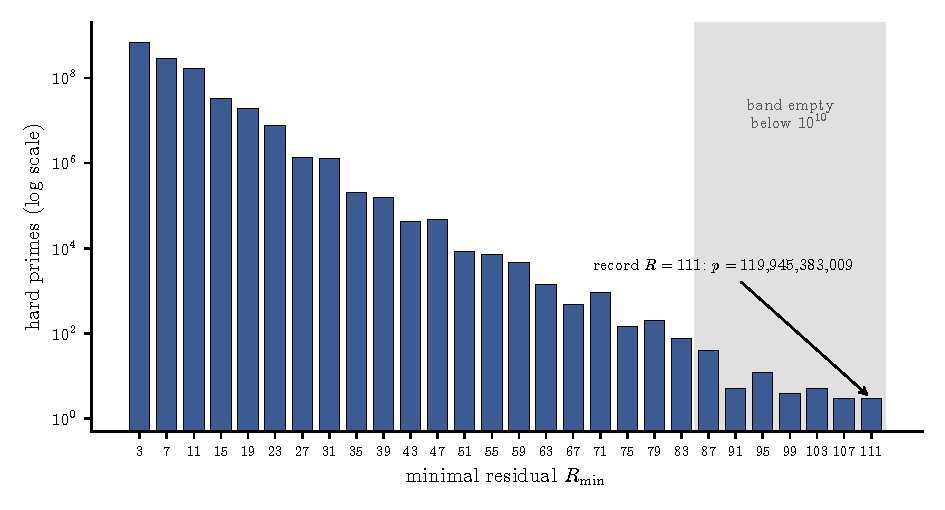
\includegraphics[width=\linewidth]{fig_minR_hist}
\caption{The data of Table~\ref{tab:dist} on a logarithmic count
scale. The head is dominated by $R = 3, 7, 11$; the tail thins
geometrically; the shaded band $87$--$111$ was empty below
$10^{10}$, and its population at $10^{11}$ and $10^{12}$ followed the
calibrated prediction (see the prediction bullet below), including
the move of the maximum from $R = 107$ to $R = 111$.}
\label{fig:hist}
\end{figure}

Three features of the distribution deserve comment.\nopagebreak
\begin{itemize}
\item \textbf{The maximum moves at $10^{12}$.} Throughout
  $10^7 \le x \le 10^{11}$ --- five successive orders of magnitude
  --- the maximal minimal residual over hard primes $p \le x$ stood
  at $R = 107$, attained by the single prime
  $8{,}803{,}369 < 10^7$. At $10^{12}$ it is
  $R_{\max} = 111$, attained by three primes, the least being
  \[
    p \;=\; 119{,}945{,}383{,}009 \;\equiv\; 529 \!\!\pmod{840},
  \]
  for which every admissible $R \le 107$ fails and $R = 111$
  certifies with $a = (p+111)/4 = 29{,}986{,}345{,}780$. The old
  record $107$ also ceased to be unique, acquiring three further
  primes in the same decade. The prime $8{,}803{,}369$ is
  extremal for a closely related statistic as well: in independent
  contemporaneous work, Bello-Hern\'andez, Benito and
  Fern\'andez~\cite{BBF} report it as the largest ``survivor''
  below $10^7$ in a $k \equiv 3 \pmod 4$ divisor sieve, requiring
  $k = 107$ there too. In the
  language of Corollary~\ref{cor:J}, $8{,}803{,}369$'s $27$ shifted
  values contain
  only $43$ distinct odd primes (typical: $45$--$52$), and $81\%$ of
  them satisfy $\smash{\legendre{p}{q}} = +1$ (typical: $44$--$60\%$)
  --- an extreme value of exactly the statistic
  Theorem~\ref{thm:J} identifies as governing joint failure. We
  attach no significance level to this: the prime was selected
  \emph{because} it was the record, so its extremeness in a
  correlated statistic is expected rather than surprising. The
  observation is
  descriptive --- it says what a record prime looks like
  mechanically, not that its existence is improbable.
\item \textbf{A prediction, and what it was worth.} The \emph{calibrated
  independence model} treats the per-residual failure events as
  independent across $R$, with per-residual failure rates fitted from
  the complete $10^9$ solvability masks and a single deep-tail
  correlation factor calibrated on the $R > 83$ counts; it is a
  heuristic, not a theorem, and its role is to make falsifiable
  predictions. Below $10^{10}$ no prime had
  minimal $R \in \{87, 91, 95, 99, 103\}$; the model
  attributed this gap to small-number statistics (expected counts
  $\le 0.12$ per value at $10^9$) and predicted that deep-tail primes
  (failing every $R \le 83$) land at $87, 91, 95, 99, 103, \ge 107$
  with probabilities $0.53, 0.11, 0.22, 0.03, 0.05, 0.06$ (the last
  being the total mass at or beyond $107$). Between
  $10^{10}$ and $10^{11}$ the five values acquired $8, 3, 5, 1, 1$
  primes respectively (all in $(1.3 \times 10^{10}, 10^{11})$), and
  none passed
  $103$; that distribution was \emph{consistent} with the prediction
  ($\chi^2 \approx 1.3$) but, on $19$ points with several expected
  cells below $5$, had little power to discriminate. The model's
  sharper commitment was about \emph{when the record would move}:
  the mass at or beyond $107$ was put at $6\%$ per deep-tail prime,
  which with the deep-tail growth rate places the first
  record-breaking prime in the decade $10^{11}$--$10^{12}$. It broke
  there, at $R = 111$. The deep tail now holds $73$ primes with
  $R_{\min} \ge 87$ against $19$ a decade earlier, distributed
  $40, 5, 12, 4, 5, 4, 3$ over $87, \dots, 111$. A model fitted at
  $10^9$ thus predicted, before the computation, both the filling of
  a band that was empty at the time and the decade in which the
  maximum would move for the first time in five orders of magnitude.
\item Among all $1{,}587{,}581$ hard primes below $10^9$, exactly
  \emph{four} admit a unique working residual $\le 107$
  ($8{,}803{,}369$ with $107$; $142{,}361{,}209$ with $59$;
  $287{,}567{,}281$ with $83$; $794{,}037{,}841$ with $63$) --- the entire
  obstruction to a shorter covering list. A greedy cover of the full
  solvability table uses $18$ residuals; a packing argument gives a lower
  bound of $12$.
\end{itemize}

\subsection{Calibration of the base case of Theorem~\ref{thm:FG}}

The proportion of hard primes failing both $R = 3$ and $R = 7$, multiplied
by $\log x$, is constant to within $1\%$ across three decades of the
$10^9$ data (Table~\ref{tab:calib}).

\begin{table}[ht]
\centering
\begin{tabular}{lccccc}
\toprule
bin ($p \sim$) & $10^6$ & $10^7$ & $6 \times 10^7$ & $2.5 \times 10^8$ & $10^9$ \\ \midrule
density $\times \log x$ & 5.14 & 5.19 & 5.18 & 5.17 & 5.16 \\
\bottomrule
\end{tabular}
\caption{The proportion of hard primes near $x$ that fail both
$R = 3$ and $R = 7$, multiplied by $\log x$, in five bins spanning three decades
of the $10^9$ data ($x$ is the bin's representative value). Constancy of the product is the decay
rate predicted by the base case of Theorem~\ref{thm:FG}.}
\label{tab:calib}
\end{table}

That is, the joint exceptional density is $\approx 5.17 / \log x$:
the decay matches the order predicted by the base case of
Theorem~\ref{thm:FG}, and $5.17$
estimates the (conjectural) Selberg--Delange constant. The exceptional
set is density zero but decays slowly: $26.5\%$ of hard primes below
$10^9$ fail both residuals; all are settled by deeper residuals of the
list. The fitted per-residual decay exponents are consistent with the
sieve prediction $\kappa = \tfrac12$ where exact criteria exist:
$\hat\kappa = 0.539$ for $R = 7$, and $\hat\kappa = 0.387$ for
$R = 3$, where the short fitting range and Selberg--Delange lower-order
terms bias the exponent downward.

\subsection{Failure taxonomy}

Sampling the complete solvability table at $10^9$: failures at $R = 7$
are $100\%$ character failures (as Theorem~\ref{thm:Ap} requires); at $R = 11$,
$89.7\%$ character failure and $10.3\%$ the budget pattern of
Theorem~\ref{thm:App}(b); the character-failure share broadly decreases with
$\varphi(R)$ (e.g.\ $51\%$ at $R = 103$, though not monotonically), as
hitting one specific class among
$\varphi(R)$ grows harder while the character dichotomy stays binary.
Taken together, the data of this section matches the framework of
Sections~\ref{sec:obstruction}--\ref{sec:sieve}: each distributional
feature --- the head, the geometric tail, the once-empty band, the
static record --- has a structural or heuristic explanation (the exact
criteria for the head; the calibrated model, built on the sieve
dimensions, for the tail and the band; Theorem~\ref{thm:J} for the
record).

\section{The sieve chain and its ceiling}\label{sec:context}

\subsection{The chain}\label{sec:sieve}

We now prove the chain of Theorem~\ref{thm:FG}, beginning with the
base case, and then Lemma~\ref{lem:S}, its unconditional upgrade
Theorem~\ref{thm:S}, the aggregate identities, and the density
reduction.

\begin{proof}[Proof of Theorem~\ref{thm:FG}, base case $\{3,7\}$]
\emph{Step 1 (exact criteria).} Let $p$ be a hard prime and set
$n = (p+3)/4$, so that $(p+7)/4 = n + 1$: \emph{the two shifted forms are
consecutive integers}. By Theorems~\ref{thm:A} and~\ref{thm:Ap}, $p$ is
exceptional (both residuals fail) precisely when
\[
  n \ \text{has no prime factor} \equiv 2 \pmod 3
  \quad\text{and}\quad
  n + 1 \ \text{has no prime factor} \equiv 3, 5, 6 \pmod 7,
\]
with $p = 4n - 3$ prime.

\emph{Step 2 (congruence bookkeeping).} Fix one of the six hard classes
$h \bmod 840$; then $n \equiv (h+3)/4 \pmod{210}$ is fixed, and the
conditions at the primes $2, 3, 5, 7$ are determined by the class (in
particular $3 \nmid n$ and $7 \nmid n+1$ automatically). It suffices to
bound each class and sum.

\emph{Step 3 (containment in a sifted set).} Let $z = x^{1/10}$. After
discarding the $O(z)$ primes $p \le z$, every exceptional $p$ gives
$n \le (x+3)/4$, $n \equiv n_0 \pmod{210}$, such that for every prime $q$
with $7 < q \le z$:
\begin{itemize}
\item[(a)] $q \equiv 2 \pmod 3 \implies n \not\equiv 0 \pmod q$;
\item[(b)] $q \equiv 3, 5, 6 \pmod 7 \implies n \not\equiv -1 \pmod q$;
\item[(c)] $q \nmid 4n - 3$ \quad (since $4n - 3 = p$ is prime, $p > z$).
\end{itemize}
Conditions (a), (b) only use ``no forbidden factor up to $z$'', which is
implied by the full criteria --- an upper bound needs no more.

\emph{Step 4 (sieve of dimension 2).} This is a standard upper-bound
sieve for the three linear forms $n$, $n+1$, $4n - 3$, with sifting
function
\[
  \omega(q) \;=\; \mathbf{1}_{q \equiv 2 (3)}
    \;+\; \mathbf{1}_{q \,\mathrm{NQR}\, (7)} \;+\; 1
  \qquad (q > 7),
\]
whose forbidden classes $0, -1, 3 \cdot 4^{-1} \bmod q$ are pairwise
distinct for $q \nmid 21$. By Dirichlet, $\omega$ has average $\kappa =
\tfrac12 + \tfrac12 + 1 = 2$ in the Halberstam--Richert sense
$\sum_{q \le w} \omega(q) \log q / q = \kappa \log w + O(1)$. The
Fundamental Lemma of sieve theory (see~\cite[Thm.~2.5]{HalberstamRichert}
and~\cite[Ch.~6]{FriedlanderIwaniec}) with $z = x^{1/10}$ bounds
the exceptional set $E(x)$ of hard primes $p \le x$ failing both
residuals:
\[
  \#E(x) \;\ll\; x \prod_{7 < q \le z} \Bigl(1 - \frac{\omega(q)}{q}\Bigr)
  \;\asymp\; x \,(\log z)^{-1} (\log z)^{-1/2} (\log z)^{-1/2}
  \;\asymp\; \frac{x}{(\log x)^2},
\]
by Mertens' theorem and its arithmetic-progression form. Summing over the
six classes preserves the bound. The higher exponents of the chain are
deduced after Lemma~\ref{lem:S} below.
\end{proof}

The verification behind Lemma~\ref{lem:S} reduces to finitely many
checks through the following elementary but load-bearing observation,
which we isolate for scrutiny.

\begin{lemma}[monotonicity reduction]\label{lem:mono}
For a class multiset $C$ (classes $v$ with multiplicities $\mu_v$) let
$D(C) = \{\sum_v e_v v : 0 \le e_v \le 2\mu_v\}$ denote the set of
attainable divisor logs (before the $p$-shifts). If $\mu_v \le \mu'_v$
for all $v$, then $D(C) \subseteq D(C')$, where $C'$ carries
multiplicities $\mu'_v$ on the same classes; likewise enlarging the support
enlarges $D$. Consequently a support $S$ carries \emph{some} failing
configuration (any multiplicities $\ge 1$ on $S$) if and only if the
all-multiplicity-one configuration on $S$ fails.
\end{lemma}

\begin{proof}
Any admissible exponent vector for $C$ is admissible for $C'$, giving
the inclusions. If a configuration on $S$ with multiplicities
$\mu_v \ge 1$ fails, the target lies outside $D(C)$, hence outside the
subset $D(C_1)$ attained at multiplicities one --- so $C_1$ fails too;
the converse inclusion is trivial. The same argument applies verbatim
after adjoining the $p$-shifts.
\end{proof}

\begin{proof}[Proof of Lemma~\ref{lem:S}]
By Lemma~\ref{lem:mono} it suffices to check that for every support of
size $(R-1)/2$ over the nonzero discrete logs and every class of
$p \bmod R$, the target is reachable already at minimal multiplicities
(exponent budget $2$ per class, $p$-budget $2$); success there kills
every configuration on every superset support at any multiplicities.
The check deliberately ignores the consistency relation
$\prod(\text{classes}) \equiv 4^{-1}p$: it therefore examines a
\emph{superset} of the realizable configurations, and can only
overstate the failing supports --- the lemma is conservative. For $R = 19, 23$ a
direct enumeration of all $(R-1)\binom{R-2}{(R-1)/2}$
(support, class of $p$) pairs suffices
($437{,}580$ resp.\ $7{,}759{,}752$ pairs; code:
\texttt{theory.verify\_support\_bound}). For the larger residuals the
binomial count explodes, and the check is instead performed by a subset
dynamic program (\texttt{theory.verify\_support\_bound\_dp}): fold all
supports into a table mapping each reachability mask to the maximal
support size achieving it --- valid because, by the same monotonicity,
failure at any multiplicities implies failure at multiplicity one. The
realized masks are heavily structured, so the state count stays
tractable ($3{,}001$ states at $R = 31$ against $77.6$~million supports;
$19{,}530{,}971$ states at $R = 107$, $331$ seconds). All twelve
residuals verify with zero violations; exact state counts are tabulated
in Table~\ref{tab:components}. The bound is tight: the all-residue
(character failure) configurations occupy exactly $(R-3)/2$ nonzero classes.
\end{proof}

Theorem~\ref{thm:S} is a statement of the critical-number literature,
and we should say so before proving it. The \emph{critical number}
$\mathrm{cr}(G)$ of a finite abelian group is the least $t$ such that
every $A \subseteq G \setminus \{0\}$ with $|A| \ge t$ has
$\Sigma(A) = G$, where $\Sigma(A)$ is the set of subset sums.
Diderrich and Mann~\cite{DiderrichMann} proved that
$\mathrm{cr}(G) = |G|/2$ for every abelian $G$ of even order, with
exactly four exceptions --- $\mathbb{Z}/4$, $\mathbb{Z}/6$,
$\mathbb{Z}/8$ and $\mathbb{Z}/2 \times \mathbb{Z}/4$ --- and the
determination for all finite abelian groups was completed by Freeze,
Gao and Geroldinger~\cite{FGG}; see also
Gao--Hamidoune--Llad\'o--Serra~\cite{GHLS} for the covering form.
Since $M(S) \supseteq \Sigma(S)$, parts (i) and (iii) of
Theorem~\ref{thm:S} follow from those theorems wherever they apply,
and the extremal family (the nonzero even classes) is theirs. More
precisely $M(S) = \Sigma(S \uplus S)$, the set of subsequence sums of
the sequence in which each element of $S$ occurs twice, so everything
in this subsection and the next lives inside the zero-sum /
Davenport-constant circle of ideas
(see~\cite[Ch.~6, 16]{Grynkiewicz}).

Three things justify giving the proof anyway. First, the exceptions
have to be handled, and the exponent budget removes them. In the
residual setting $G = (\mathbb{Z}/R)^*$, and among admissible
$R \equiv 3 \pmod 4$ the exceptional groups occur at exactly
$R = 7$ (giving $\mathbb{Z}/6$) and $R = 15$ (giving
$\mathbb{Z}/2 \times \mathbb{Z}/4$); no admissible $R$ has
$\varphi(R) = 4$. At those two residuals the Diderrich--Mann bound
$|S| \le g/2 - 1$ is false for $\Sigma(S)$ --- supports of size
$g/2$ with $\Sigma(S) \ne G$ exist --- but true for $M(S)$, because
allowing each class twice is exactly enough to close the gap. The
proof below gives $|S| \le g/2 - 1$ for $M$ at every even-order $G$
with no exceptions, so the sieve dimension $\tfrac12$ is available at
\emph{every} admissible residual. (At $R = 7$ and $R = 15$ this is
belt and braces: Theorems~\ref{thm:Ap} and~\ref{thm:R15} give an
exact criterion there in any case.) Second, the summands here are not
arbitrary: each factor class contributes the bounded-exponent set
$\{1, v, v^2\}$, and the derivation below yields the quantitative
form we need --- a single prescribed target, bounds uniform in $R$,
and the involution bookkeeping of part (iii) --- directly. Third, it
is short, and it is what the Lean development formalizes.

\begin{proof}[Proof of Theorem~\ref{thm:S}]
(i) Write $M = A_1 + \cdots + A_k$ with $A_i = \{0, v_i, 2v_i\}$,
$k = |S|$, and let $H = \mathrm{Stab}(M) = \{h : M + h = M\}$, a
subgroup of $\mathbb{Z}/d$. Kneser's addition theorem
\cite{Kneser} (in the many-summand form obtained by iterating
\cite[Thm.~5.5]{TaoVu}) gives
\[
  |M| \;\ge\; \sum_{i=1}^{k} |A_i + H| \;-\; (k-1)\,|H|.
\]
\emph{Case $H = \{0\}$.} Every $|A_i| = 3$, except that the (at most
one) index $i$ with $v_i = d/2$ has $|A_i| = 2$ (there $2v_i = 0$); so
$|M| \ge (3k - 1) - (k - 1) = 2k$. Since $M \ne \mathbb{Z}/d$,
$2k \le d - 1$, and $d$ even forces $k \le d/2 - 1$.
\emph{Case $|H| = h > 1$.} $M$ is a union of $H$-cosets and
$M \ne \mathbb{Z}/d$, so $|M| \le d - h$. Split
$k_0 = |S \cap H| \le h - 1$ (distinct nonzero elements of $H$) and
$k_1 = k - k_0$. For $v \in H$, $|A_v + H| = h$; for $v \notin H$,
$A_v + H \supseteq H \cup (v + H)$, so $|A_v + H| \ge 2h$. Kneser's
bound gives $d - h \ge h(k_0 + 2k_1 - k + 1) = h(k_1 + 1)$, so
$k_1 \le d/h - 2$ and $k \le (h-1) + (d/h - 2) = h + d/h - 3$. For
every divisor $h$ with $2 \le h \le d/2$, the quadratic
$h^2 - (\tfrac d2 + 2)h + d \le 0$ (its roots are $2$ and $d/2$), i.e.\
$h + d/h - 3 \le d/2 - 1$. Tightness: for $S$ the nonzero even
classes, $M(S)$ is the even subgroup and $|S| = d/2 - 1$.

(ii) In discrete-log coordinates on $(\mathbb{Z}/R)^* \cong
\mathbb{Z}/d$, $d = R - 1$, the divisor classes of $m^2$ contain the
set $M(S)$ over the nonzero support $S$ of $(p+R)/4$ at exponent
budget $2$ per class (Lemma~\ref{lem:mono}: multiplicities $\ge 1$
only enlarge budgets). If $|S| \ge d/2$, part (i) forces
$M(S) = \mathbb{Z}/d$: every class --- in particular the target $-m$
--- is a divisor class of $m^2$, without invoking the $p$-powers, and
\eqref{eq:cert} holds. Contrapositively, failure at $R$ forces
$|S| \le d/2 - 1 = (R-3)/2$, which is the conclusion of
Lemma~\ref{lem:S} for arbitrary $R$.

(iii) The argument in (i) never used cyclicity. In a finite abelian
$G$ of even order $g$: in the $H$-trivial case each involution
$v \in S$ has $|\{1, v, v^2\}| = 2$, so
$|M| \ge (3k - t) - (k - 1) = 2k - t + 1$ and $M \ne G$ gives
$k \le \lfloor (g + t - 2)/2 \rfloor$; the $|H| = h > 1$ case is
verbatim, giving $k \le h + g/h - 3 \le g/2 - 1$ over proper
subgroups. For $G = (\mathbb{Z}/R)^*$, $t = 2^{\omega(R)} - 1$; with
$\omega(R) \le 2$, $t \le 3$ and the bound is $\le g/2$, so failure
forbids at least $(g - 1) - g/2 = \varphi(R)/2 - 1$ non-identity unit
classes --- dimension $\ge \tfrac12 - 1/\varphi(R)$. The general-$t$
clause is the same computation without the specialization: failure
forbids at least $(g-1) - (g+t-2)/2 = (g-t)/2$ non-identity classes
(minus one when the max is attained by $g/2-1$), and
$2^{\omega(R)} \le R^{O(1/\log\log R)} = R^{o(1)}$ gives the stated
$0.44$ threshold beyond an absolute bound. The upgrade to
$\varphi(R)/2$ forbidden classes for $R \le 107$ is the enumeration
cited in the statement: the maximum support of a proper product-set is
exactly $g/2 - 1$ for every composite admissible $R \le 107$
(\texttt{theory.kneser\_support\_general}; e.g.\ $R = 95$: $g = 72$,
maximum $35$ over $583{,}455$ realizable product-sets). That
enumeration is a proof component of the $R \le 107$ clause, on the
same footing as the checks of Remark~\ref{rem:computer}; the
$\tfrac12 - 1/\varphi(R)$ tier needs Kneser alone.
\end{proof}

\begin{remark}
Theorem~\ref{thm:S}(ii) is strictly stronger than what the sieve
needs: at support $\ge (R-1)/2$ \emph{every} class is reachable, for
every target and every $p$. The strong form is also confirmed
numerically (\texttt{theory.verify\_support\_bound\_strong}): the
maximum support of a non-full reachability mask equals $(R-3)/2$
exactly at every prime residual checked. Lemma~\ref{lem:S} and its
dynamic-program verifications stand as independent machine
confirmations of special cases (and remain the form carried by the
Lean development).
\end{remark}

\begin{proof}[Proof of Theorem~\ref{thm:FG}, higher exponents]
Write $n = (p+3)/4$; the relevant forms are $n$, $n+1$, $n+2 = (p+11)/4$,
$n+3 = (p+15)/4$, $n+4 = (p+19)/4$, and $4n-3 = p$. Joint failure of
$\{3,7,11\}$ implies, by Theorems~\ref{thm:A}, \ref{thm:Ap},
\ref{thm:App}: $n$ free of primes $\equiv 2 \pmod 3$; $n+1$ free of
non-residues mod $7$; and, splitting by the two cases of
Theorem~\ref{thm:App}: \emph{branch (a)} --- $n+2$ free of the five
non-residue classes mod $11$ (density $\tfrac12$); \emph{branch (b)} ---
$n+2$ free of the six classes $\{4,5,7,8,9,10\}$ mod $11$ (density
$\tfrac35$). Each branch is a four-form sieve problem of dimension
$1 + \tfrac12 + \tfrac12 + \tfrac12 = \tfrac52$, resp.\
$1 + \tfrac12 + \tfrac12 + \tfrac35 = \tfrac{13}{5}$. Since
$\tfrac{13}{5} > \tfrac52$, the budget branch contributes
$O(x/(\log x)^{13/5}) = o(x/(\log x)^{5/2})$:
the bound is the maximum of the branch exponents, attained by the
character branch (a). The Fundamental Lemma applied to each branch gives
$O(x/(\log x)^{5/2})$ in total.

Adjoining $R = 15$: by Theorem~\ref{thm:R15}, failure at $15$ is the
single condition ``$n + 3$ free of the four classes
$\{7, 11, 13, 14\}$ mod $15$'' --- one branch, density
$\tfrac{4}{8} = \tfrac12$ over the $\varphi(15) = 8$ unit classes ---
raising each combined branch to dimension $\ge 3$: joint failure of
$\{3, 7, 11, 15\}$ is $O(x/(\log x)^3)$.

For $\{3,7,11,15,19\}$, Theorem~\ref{thm:S} (equivalently, at this
residual, Lemma~\ref{lem:S}) splits failure at $19$ into
finitely many maximal-support branches, each forbidding an explicit set
of at least $9$ of the $18$ unit classes mod $19$ on $n+4$ --- dimension
$\ge \tfrac12$. Crossing with the branches at $11$ leaves finitely many
combined branches, each a six-form problem of dimension $\ge \tfrac72$
(those involving the budget case at $11$ have dimension
$\ge \tfrac{31}{10} + \tfrac12 > \tfrac72$
and are again lower-order); the
forbidden residues of the six forms are pairwise distinct for $q > 19$,
smaller primes being absorbed into the congruence class of $n$. Summing
the finitely many branches gives $O(x/(\log x)^{7/2})$.

The general case is identical: for a finite admissible list
$\mathcal{P}$ (prime, or composite with $\omega(R) \le 2$), the forms
$n + (R-3)/4$, $R \in \mathcal{P}$, are distinct integer shifts of
$n$; Theorems~\ref{thm:A}, \ref{thm:Ap}, \ref{thm:App}, \ref{thm:R15}
handle $R = 3, 7, 11, 15$ and Theorem~\ref{thm:S} handles every other
residual (part (ii) for primes, part (iii) for composites), each
contributing dimension $\delta_R$ through finitely many
maximal-support branches --- $\delta_R = \tfrac12$ for primes and for
composites $\le 107$, $\delta_R = \tfrac12 - 1/\varphi(R)$ for larger
composites (the two tiers of part (iii)) --- plus $1$ for primality:
total dimension $\ge 1 + \kappa(\mathcal{P})$, with forbidden residues
pairwise distinct for $q > \max \mathcal{P}$ and smaller primes
absorbed into the congruence class of $n$. For the fifteen primes up
to $107$ this gives
exponent $\tfrac{17}{2}$; for the full $27$-element admissible list,
$\tfrac{29}{2}$.
\end{proof}

\begin{proof}[Proof of Proposition~\ref{prop:agg}]
$k = a p^2$ divides $m^2 = p^2 a^2$ and $k \equiv -m$ if and only if
$a p^2 \equiv -p a$, i.e.\ $p \equiv -1 \pmod R$; $k = a^2 p$ divides
$m^2$ and $a^2 p \equiv -p a$ if and only if $a \equiv -1$, i.e.\
$p \equiv -4 \pmod R$ by \eqref{eq:star}. Integrality of $b, c$ is
automatic. Scanning all shapes $k = a^j p^i$ ($j, i \le 2$) yields no
further $p$-only condition. The failure of both families states that the
two forms $(p+1)/2$ and $p+4$ (in $n$: $2n-1$ and $4n+1$) are free of
primes $\equiv 3 \pmod 4$ --- two further sifting conditions of
dimension $\tfrac12$ each on forms distinct from all previous ones.
\end{proof}

Empirically the two families alone cover $74\%$ of hard primes below
$10^9$ --- and none of the four primes of Section~\ref{sec:comp} that
admit a unique working residual $\le 107$.

\begin{remark}\label{rem:emptiness}
By Theorem~\ref{thm:S}, every residual --- prime or composite --- adds
$\tfrac12$ to the exponent, so the chain's exponent is bounded only by
the number of residuals used; the constants $O_{\mathcal{P}}$, however,
grow with $|\mathcal{P}|$ (branch counts and the remainder term of the
Fundamental Lemma). The chain is a concrete instantiation of
Theorem~\ref{thm:D} with explicit constants. One caveat frames its
scope, and it is fundamental: no fixed finite list can be pushed to
\emph{emptiness}
by upper-bound sieving: the count bound $x/(\log x)^{\kappa}$ diverges
for every fixed $\kappa$, and extrapolating the calibration of
Section~\ref{sec:comp} to any fixed list yields a positive density
constant, i.e.\ infinitely many expected exceptional primes with the
record minimal residual growing slowly without bound. The correctly
posed remaining problem is a slowly growing bound $R_{\min}(p) \ll f(p)$,
which requires existence (lower-bound) technology beyond upper-bound
sieves.
\end{remark}

\begin{proof}[Proof of Theorem~\ref{thm:D}]
Fix $A > 0$. Choose $B = B(A)$ so large that
\begin{equation}\label{eq:divergence}
  \sum_{\substack{3 \le R \le B \\ R \equiv 3 \ (4)}} \frac{1}{\varphi(R)}
  \;\ge\; \sum_{\substack{3 \le R \le B \\ R \equiv 3 \ (4)}} \frac{1}{R}
  \;>\; A;
\end{equation}
this is possible since the reciprocal sum over the progression
$R \equiv 3 \pmod 4$ diverges, and $\varphi(R) \le R$. Let
$S(A) = \{R \equiv 3 \pmod 4 : 3 \le R \le B\}$ and
$M = 840 \cdot \prod_{R \in S(A)} R$.

Write $n = (p+3)/4$ as before, so $(p+R)/4 = n + (R-3)/4$ for each
$R \in S(A)$: a family of $|S(A)|$ integer linear forms in $n$ with
pairwise distinct shifts, together with the form $4n - 3 = p$. Set
$z = x^{1/10}$ and discard the $O(z)$ primes $p \le z$. Fix a
residue class $n \equiv n_0 \pmod M$ compatible with $p$ hard; there are
finitely many, and it suffices to bound each. Within such a class, for
every $R \in S(A)$ the quantities $t \equiv -4^{-1}p^2$ and
$p^{-1} \bmod R$ are constant, so the class set
$S_R(p) = \{t, tp^{-1}, tp^{-2}\} \bmod R$ of
Proposition~\ref{prop:succ} is a fixed nonempty set of
$t_R = t_R(n_0) \in \{1, 2, 3\}$ classes. By the contrapositive of
Proposition~\ref{prop:succ}, if every residual in $S(A)$ fails at $p$,
then for each $R \in S(A)$ the form $n + (R-3)/4$ has \emph{no} prime
factor in $S_R(p)$; and $4n - 3$, being prime and greater than $z$,
has no prime factor $\le z$.

Sift the class $\{n \le (x+3)/4 : n \equiv n_0 \ (M)\}$ by the primes
$q \le z$, $q \nmid M$. A prime $q$ forbids: the class
$n \equiv 3 \cdot 4^{-1} \pmod q$ (from the primality of $4n - 3$), and,
for each $R \in S(A)$ with $q \bmod R \in S_R(p)$, the single class
$n \equiv -\tfrac{R-3}{4} \pmod q$ (a prime factor $q$ of the form
$n + (R-3)/4$ in a guaranteed-success class cannot occur). Thus
\[
  \omega(q) \;=\; 1 \;+\;
  \#\bigl\{R \in S(A) : q \bmod R \in S_R(p)\bigr\},
\]
which is bounded by $|S(A)| + 1$; the forbidden residues of distinct
forms are pairwise distinct for $q > B$, since the shifts $(R-3)/4$
differ by less than $B$ and $q \nmid M$. For each $R$, the density of
primes $q$ with $q \bmod R \in S_R(p)$ is $t_R/\varphi(R)$ by
Dirichlet's theorem, so $\omega$ has average
\[
  \kappa \;=\; 1 + \sum_{R \in S(A)} \frac{t_R}{\varphi(R)}
  \;\ge\; 1 + \sum_{R \in S(A)} \frac{1}{\varphi(R)} \;>\; 1 + A,
\]
in the Halberstam--Richert sense, by \eqref{eq:divergence}. The
Fundamental Lemma~\cite[Thm.~2.5]{HalberstamRichert} in dimension
$\kappa$ then bounds the sifted count by
$O_{A}\!\left(x \prod_{q \le z}(1 - \omega(q)/q)\right)
 = O_A\!\left(x (\log x)^{-\kappa}\right)
 = O_A\!\left(x/(\log x)^{1+A}\right)$,
and summing over the finitely many classes $n_0 \bmod M$ preserves the
bound.
\end{proof}

\begin{remark}
Theorem~\ref{thm:D} is the strongest statement the pure sieve can give:
density $O((\log x)^{-A})$ for every $A$, but not emptiness. The
conjecture for hard primes would follow from a \emph{finite covering
hypothesis}: some finite $S$ admits, for every hard prime, a residual
$R \in S$ with \eqref{eq:cert} (the converse is not automatic --- the
conjecture bounds $R_{\min}(p)$ by $2p$, not uniformly). The data to $10^{12}$ is covered by
$S = \{3, 7, 11, \dots, 107\}$ --- yet both the calibration
(Remark~\ref{rem:emptiness}) and the conditional construction of
Section~\ref{sec:open} predict that any fixed list eventually fails.
\end{remark}

\subsection{The uniform chain}\label{sec:uniform}

Theorem~\ref{thm:D} fixes the list $S(A)$ once $A$ is fixed; letting
the list \emph{grow with $x$} is purely a question of uniformity in
the constants of Theorem~\ref{thm:FG} --- the branch count per
residual, the class modulus, and the sieve constants in growing
dimension. Auditing those constants shows the growth is affordable
for lists of length a small multiple of $\log\log x$, which yields
the strongest unconditional statement of this paper.

\begin{theorem}[uniform chain]\label{thm:U}
There are absolute constants $\varepsilon, c > 0$ and an
(ineffective) $x_0$ such that for all $x \ge x_0$,
\[
  \#\bigl\{\text{hard primes } p \le x :
  R_{\min}(p) > \varepsilon \log\log x\bigr\}
  \;\le\; x\,\exp\!\bigl(-c\,(\log\log x)^2\bigr).
\]
In particular, all but $O(x e^{-c(\log\log x)^2})$ hard primes
$p \le x$ possess an explicit, divisor-exhibited residual certificate
at some admissible $R \le \varepsilon\log\log x$ ---
unconditionally.
\end{theorem}

\begin{proof}
Write $L = \log\log x$, $B = \varepsilon L$, and let $\mathcal{R}$ be
the admissible residuals $3 \le R \le B$
($|\mathcal{R}| \sim B/4$). Discard the $O(\sqrt x)$ primes
$p \le \sqrt x$. A hard prime with $R_{\min}(p) > B$ fails every
$R \in \mathcal{R}$; we bound the count of such $p$ by a single
sieve application per \emph{branch}, as follows.

\emph{Dimensions.} Each $R \in \mathcal{R}$ contributes a sifting
dimension $\delta_R$: the exact criteria at $R = 3, 7, 11, 15$ and
Theorem~\ref{thm:S}(ii) at primes give $\delta_R = \tfrac12$;
composites $\le 107$ give $\tfrac12$ by the sharpened tier of
Theorem~\ref{thm:S}(iii); and every remaining composite --- with
\emph{no} restriction on $\omega(R)$ --- gives
$\delta_R \ge \tfrac12 - (2^{\omega(R)-1}+1)/\varphi(R) \ge 0.44$
beyond an absolute bound $R_1$, by the general-$t$ clause of
Theorem~\ref{thm:S}(iii). Hence
$\kappa := 1 + \sum_{R \in \mathcal{R}} \delta_R
\ge 1 + 0.44(|\mathcal{R}| - R_1) \ge 1 + B/10$ for $B$ large.

\emph{Branches.} For each $R$, failure confines the support of
$(p+R)/4$ to one of at most $2^{\varphi(R)}$ failing supports
$S_R$ (crudely, all subsets); fixing $(S_R)_{R \in \mathcal{R}}$
and the class $n_0$ of $n = (p+3)/4$ modulo
$\widetilde M = \mathrm{lcm}(840, \prod_{\ell \le B} \ell) =
e^{O(B)}$ costs a factor
$\prod_R 2^{\varphi(R)} \cdot e^{O(B)} = e^{O(B^2)}$ branches.

\emph{Sieve.} Within a branch, sift the integers
$n \le (x+3)/4$, $n \equiv n_0 \pmod{\widetilde M}$, by the primes
$\ell \in (B, z]$, $z = x^{1/s}$: the forbidden classes mod $\ell$
are $n \equiv 3 \cdot 4^{-1}$ (so that $p = 4n-3$ keeps no factor
$\le z$) and, for each $R$ with $\ell \bmod R$ outside $S_R$,
$n \equiv -(R-3)/4$ --- pairwise distinct for $\ell > B$, so
$\omega(\ell) \le |\mathcal{R}| + 1 < \ell/2$. The density
condition holds with the dimension $\kappa$ above and
$(\Omega)$-constant $O(B \log B)$, by Mertens' theorem in the
progressions modulo $R \le B$ (Siegel--Walfisz range, whence the
ineffective $x_0$). Apply Brun's sieve of order $r \asymp \kappa$
(\cite[Ch.~2]{HalberstamRichert}; for constants uniform in the
dimension, \cite[Thm.~6.9]{FriedlanderIwaniec}) at $s = 10r$, so
that $z^r = x^{1/10}$: since the
sifted sequence consists of \emph{integers} in a progression --- no
primality is detected anywhere --- the remainder is
$\sum_{d \le z^r} (B+2)^{\omega(d)} \ll x^{1/10} e^{O(BL)} =
x^{1/10 + o(1)}$ for a suitable absolute choice of the implied
constants, and the main term is
\[
  \ll \frac{x}{\widetilde M} \prod_{B < \ell \le z}
  \Bigl(1 - \frac{\omega(\ell)}{\ell}\Bigr)
  \;\le\; x \exp\bigl(-\kappa (L - O(\log B)) + O(B\log B)\bigr).
\]

\emph{Accounting.} Multiplying by the branch count,
\[
\begin{aligned}
  \#\{p \le x : R_{\min}(p) > B\}
  \;&\le\; e^{O(B^2)}\, x\, \exp\bigl(-\kappa L + O(B \log B) +
  O(\kappa \log B)\bigr) \\
  &\le\; x\,\exp\bigl(-BL/10 + O(B^2)\bigr),
\end{aligned}
\]
and with $B = \varepsilon L$ the exponent is
$-\varepsilon L^2/10 + O(\varepsilon^2 L^2) \le
-\varepsilon L^2/20$ for $\varepsilon$ below an absolute threshold.
\end{proof}

\begin{remark}[the constant, and the range]\label{rem:Urange}
The constant $c$ in Theorem~\ref{thm:U} is not innocuous. It
inherits the branch factor $e^{\Theta(B^2)}$ against the sieve gain
$e^{-BL/10}$, so the $\varepsilon$ below which the accounting closes
is small, and $c \asymp \varepsilon$. The bound beats the trivial
count $\asymp x/(32\log x)$ of hard primes only once
$c(\log\log x)^2 - \log\log x > \log 32$, which for small $c$
places the crossover at values of $x$ far beyond any computational
range: at $c = 10^{-2}$ one needs $\log\log x \gtrsim 350$. The
theorem is therefore asymptotic in the strict sense --- nontrivial
for all large $x$, ineffectively so (Siegel--Walfisz), and of no
numerical content in any accessible range. Its interest is
structural, and the numerical picture at accessible heights is
supplied instead by Section~\ref{sec:comp}.
\end{remark}

\begin{remark}[the ceiling, and the one lever]\label{rem:ceiling}
Theorem~\ref{thm:U} sits at the boundary set by its \emph{branch
factor}: $e^{\Theta(B^2)}$ from the crude all-subsets bound on
failing supports, against the sieve gain $e^{-BL/10}$, forces
$B \ll L$ and the ceiling $\exp(-cL^2)$. A closer audit
(Section~\ref{sec:branch}) shows the branch factor is the
\emph{only} binding wall: the class modulus
$\widetilde M = e^{O(B)}$ never multiplies the main term (the
classes partition the integers), and the Mertens/Siegel--Walfisz
inputs remain valid for $B$ up to any fixed power of $\log x$ at the
already-paid price of ineffectivity. Classifying the failing
supports into polynomially many structured branches --- the subject
of Section~\ref{sec:branch} --- would therefore raise
Theorem~\ref{thm:U} to an exceptional set
$x\exp(-(\log x)^{c_0})$ with $R_{\min} \le (\log x)^{c_0}$
(Theorem~\ref{thm:Upay}), with the family ceiling strictly below
exponent $\tfrac12$ (see the discussion there). Vaughan's bound
$x\exp(-c(\log x)^{2/3})$~\cite{Vaughan}
remains stronger as a pure density statement at every tier of this
family; what
Theorem~\ref{thm:U} adds is structural: an explicit certificate at a
small residual for almost every hard prime, a
statement mean-value methods do not address. The calibrations
$J = (\log x)^{\theta}$ of Theorem~\ref{thm:L1} remain out of reach
of every unconditional variant considered here.
\end{remark}

\subsection{The branch classification}\label{sec:branch}

Fix a prime residual $R$, $d = R - 1$, and work in the discrete-log
model of Theorem~\ref{thm:S}(i): a \emph{support}
$S \subseteq \mathbb{Z}/d \setminus \{0\}$ at exponent budget $2$
per class has reach $M(S) = \sum_{v \in S} \{0, v, 2v\}$, and $S$
\emph{fails} for a target $t$ if $t \notin M(S)$ (the $p$-budget is
absorbed as one more summand). By
Lemma~\ref{lem:mono} every failing configuration lives on a failing
support, and every failing support extends to a \emph{maximal} one
($S$ failing, $S \cup \{w\}$ succeeding for all $w$). Two facts
calibrate the problem. First, maximality forces no size
concentration: maximal failing supports exist at every size scale
from
$\Theta(\log d)$ (complete-partition constructions realizing
$M(S) = \mathbb{Z}/d \setminus \{t\}$, a \emph{singleton miss}) up
to the extremal $d/2 - 1$. Second, \emph{enumerating} them is
hopeless:

\begin{theorem}[branch count blow-up]\label{thm:Mcount}
There is $c > 0$ such that for every large even $d$, the number of
maximal failing supports for the target $t = -1$ in $\mathbb{Z}/d$
is at least $2^{c\sqrt d}$: the supports
$[1, r] \cup T' \cup \{X\}$, $T' \subseteq [r+1, 2r]$,
$|T'| = \lceil r/2 \rceil$, $r = \lceil\sqrt{d/4}\,\rceil$, with $X$
completing the sum to $d/2 - 1$, are pairwise distinct
complete partitions (for $d$ large, $X > 2r$, so $X$ collides with
no other part and $T'$ is recoverable from the support; the chain
condition at the part $X$ reduces to $d/2 - 2 \le 3r(r+1)$, which
holds since $r^2 \ge d/4$), and each
has reach exactly
$\mathbb{Z}/d \setminus \{-1\}$, hence is maximal failing.
\end{theorem}

The exponential-in-$\sqrt d$ order is not a surprise: the objects
constructed are complete partitions with distinct parts, whose total
count is $\exp(\Theta(\sqrt n))$ classically
(Andrews--Beck--Hopkins~\cite{ABH}). What
Theorem~\ref{thm:Mcount} records is the version adapted to
$\mathbb{Z}/d$ and to maximality, because that is what rules out
enumeration. A useful classification must therefore produce
\emph{containers} --- polynomially many structured sets covering all
failing supports. The kernel (periodic) case is under complete
control, by the standard stabilizer/quotient reduction that drives
the critical-number literature
(see~\cite[Ch.~6]{Grynkiewicz}); we state it in the form and with the
size bookkeeping we need, and claim no novelty in the mechanism.

\begin{theorem}[kernel branch; lossless reduction]\label{thm:Mkernel}
Let $S$ fail for $t$ and $H = \mathrm{Stab}(M(S)) \ne \{0\}$, and
write $\varphi_H \colon \mathbb{Z}/d \to \mathbb{Z}/\bar d$. Then
$t \notin M(S) + H$, the projection
$\bar T = \varphi_H(S \setminus H)$ is a failing support for
$\bar t = \varphi_H(t) \ne 0$ at the same budget, and
$S \subseteq (H \setminus \{0\}) \cup \varphi_H^{-1}(\bar T)$; if
$S$ is maximal then moreover $H \setminus \{0\} \subseteq S$.
Iterating: every failing support of $\mathbb{Z}/d$ is contained in
$\psi^{-1}(\{0\} \cup T') \setminus \{0\}$ for a composed quotient
$\psi \colon \mathbb{Z}/d \to \mathbb{Z}/d'$ and an
\emph{aperiodic maximal} failing support $T'$ downstairs, and this
container has at most $\lfloor d/2 \rfloor - 1$ elements. (The
support bound extends to odd moduli, as needed for the quotients:
for odd $\bar d$ no summand is degenerate, so in the aperiodic case
Kneser's bound gives
$|T| \le (\bar d - 3)/2$; for nontrivial stabilizer of order $h$
the count is $\le h + \bar d/h - 3 \le \bar d/3 \le (\bar d - 3)/2$
for $\bar d \ge 9$, smaller odd $\bar d$ having no proper
nontrivial subgroups.)
\end{theorem}

\begin{proof}
$M + H = M$ gives $H \subseteq M$ and $t \notin M + H$ (else
$t \in M$), so $\bar t \ne 0$. The projection
$\varphi_H(M(S)) = \sum_{v} \{0, \bar v, 2\bar v\}$ contains
$M(\bar T)$ computed downstairs at budget $2$ (collisions only
enlarge budgets; Lemma~\ref{lem:mono}), and $H$-saturation of
$M(S)$ turns $t \notin M(S)$ into $\bar t \notin M(\bar T)$: $\bar
T$ fails. The containment is definitional. For maximality: any
$w \in H \setminus (S \cup \{0\})$ has $A_w \subseteq H$, so
$M(S \cup \{w\}) = M(S) + A_w = M(S)$ still fails --- $w$ must
already lie in $S$. Iterate on the quotient (strong induction on
$d$, extending $\bar T$ to a maximal support downstairs first); the
size bookkeeping per step is
$(h - 1) + h\,|T'| \le h - 1 + h \lfloor (\bar d - 2)/2 \rfloor
\le d/2 - 1$, exact at even $\bar d$, with strict inequality at odd
$\bar d$.
\end{proof}

The open core is the aperiodic case. All the evidence points to one
container shape --- a coset-progression \emph{window}: for
$K \le \mathbb{Z}/d$, a unit direction and a circular window $W$ of
quotient classes, set
$C(K, W) = \varphi_K^{-1}(\{0\} \cup W) \setminus \{0\}$. The
family $\{C(K, W) : |C(K, W)| \le \lfloor d/2 \rfloor - 1\}$ has
fewer than $d^3$ members (a container is determined by the kernel
size $\kappa \mid d$, a unit direction, a window start, and a window
length $\le \bar d/2$: at most
$\sum_{\kappa \mid d} \bar d^{\,3}/2 \le \zeta(3)d^3/2$ choices).

\begin{conjecture}[aperiodic branch classification]\label{conj:A}
Every maximal failing support $S$ with
$\mathrm{Stab}(M(S)) = \{0\}$ for a target $t$ in $\mathbb{Z}/d$
satisfies $S \subseteq C(K, W)$ for some window container with
$|C(K, W)| \le \lfloor d/2 \rfloor - 1$.
\end{conjecture}

The evidence: exhaustive verification for \emph{all} moduli
$d \le 60$ and all targets ($24.25$ million orbit-weighted maximal
supports; zero violations; the bound
$\lfloor d/2 \rfloor - 1$ is attained, hence optimal); exhaustive
verification at $d = 72$, the smallest \emph{non-Haj\'os} cyclic
order --- the one place aperiodic factorization pathologies could
first appear --- over all $11$ target orbits and $14.99$ million
maximal supports, with extensive stratified sampling (including
supports seeded from explicit aperiodic de~Bruijn factorizations of
$\mathbb{Z}/72$) at every non-Haj\'os order up to $240$; independent
verification in the residual model at
$R = 19, 23, 31, 43, 47, 59$ ($495{,}782$ maximal supports at
$R = 59$) and
at the composite moduli $R = 15, 35, 39$ (entry point
\texttt{erdos\_straus.branch\_enum}; archived); a proved
subfamily (the signed complete partitions, windows with room to
spare); and a rank-$2$ witness
($S = \{11, 17, 19, 29\} \subseteq \mathbb{Z}/30$, a singleton miss
contained in no short one-dimensional window but in a
$K = \langle 10 \rangle$ window container of size $14$) showing the
subgroup component of the shape is necessary. Combining
Theorem~\ref{thm:Mkernel} with Conjecture~\ref{conj:A} in the
quotients (windows pull back to windows along composed quotients):

\begin{theorem}[container form; conditional on
Conjecture~\textup{\ref{conj:A}}]\label{thm:Mcont}
Every failing support for $(d, t)$ is contained in one of fewer
than $d^3$ explicit window containers of size
$\le \lfloor d/2 \rfloor - 1$; hence failure of residual $R$
confines the factor classes of $(p+R)/4$ to one of $O(R^3)$
branches, each forbidding at least half the nonzero classes ---
sieve dimension $\tfrac12$ per residual, with the branch count
reduced from $2^{\varphi(R)}$ to $O(R^3)$.
\end{theorem}

\begin{theorem}[conditional uniform chain, polylog
tier]\label{thm:Upay}
Assume Conjecture~\ref{conj:A} (for all moduli). Then there is an
absolute $c_0 > 0$ such that all but
$O\bigl(x \exp(-(\log x)^{c_0})\bigr)$ hard primes $p \le x$
satisfy $R_{\min}(p) \le (\log x)^{c_0}$.
\end{theorem}

\begin{proof}[Proof sketch]
Rerun the proof of Theorem~\ref{thm:U} with list length
$B = (\log x)^{\theta}$. The branch factor over the list drops from
$e^{\Theta(B^2)}$ to $\prod_{R \le B} O(R^3) =
e^{(3+o(1)) \cdot \frac{B}{4}\log B}$; the class conditioning
never multiplies the main term (the classes partition the sifted
integers, so the per-class main terms resum); and Siegel--Walfisz
covers the Mertens-in-progressions inputs for moduli up to any
fixed power of $\log x$. The per-residual balance is then a sieve
gain $\delta(1-\theta)L$ against a branch-and-slop cost
$(3 + c_M)\theta L$, where $L = \log\log x$, $\delta = \tfrac12$,
and $c_M$ collects the per-residual slop --- the
Mertens-in-progressions constants, the discarded initial segment
$\ell \le B$ of sieving primes, and the $(\Omega)$-condition
constant, together of order $1$. This is
admissible for every
$\theta < \delta/(3 + c_M + \delta)$ --- with the constants proved
here, any $\theta$ below roughly $1/9$. The family ceiling sits
strictly below $\tfrac12$: no container scheme of this shape has
fewer than ${\sim}d$ members (distinct progression directions
already require distinct containers), so the count exponent is at
least $1$ and the balance caps $\theta$ at
$\delta/(1 + c_M + \delta) < \tfrac13$ --- consistent with, and
sharper than, the $\exp(-(\log x)^{1/2+o(1)})$ outer ceiling of the
wider method family, itself short of Vaughan's $2/3$. A
quasi-polynomial classification ($d^{O(\log d)}$ containers) would
still give exceptional sets
$x\exp(-\exp(c\sqrt{\log\log x}))$, past every
$\exp(-C(\log\log x)^A)$.
\end{proof}

Conjecture~\ref{conj:A} is thus a single well-posed question of
additive combinatorics --- a container theorem of Kneser--Freiman
type for bounded-exponent subset sums --- standing between
Theorem~\ref{thm:U} and its polylog tier. Where its difficulty lives
can now be pinned exactly. Near-critical Kneser analysis is
\emph{vacuous} here (aperiodic failing supports with $|S| \ge 3$ are
never Kneser-tight --- the governing mechanism is exact covering by
complete sequences, not small doubling); the singleton-miss
supports satisfy the symmetry $2\sum_{v \in S} v = 2t$, which pins
their windows (and at \emph{odd} moduli singleton misses do not
exist at all: the miss set always has even size, so the floor family
there is $|F| = 2$, auto-maximal and window-shaped). The one
mechanism previously feared --- chaining of \emph{punctured}
(cofinite) intermediate reaches, where direction information
degenerates and non-Hajós factorization pathologies could hide ---
is provably empty:

\begin{proposition}[$\beta$-vacuity]\label{prop:betavac}
Let $S$ fail for $t$ in $\mathbb{Z}/d$, let $v \in S$, and suppose
the deletion step at $v$ is Kneser-critical
($|M(S)| = |M(S \setminus \{v\})| + 2$) of punctured type: the two
new elements are isolated punctures of the complement. Then
$F - v = F$ for the miss set $F = \mathbb{Z}/d \setminus M(S)$, so
$v \in \mathrm{Stab}(M(S))$. In particular, for an \emph{aperiodic}
maximal failing support every critical deletion step is of window
($\alpha$) type.
\end{proposition}

\begin{proof}
Write $A = M(S \setminus \{v\})$ and
$\mathbb{Z}/d \setminus A = F \sqcup \{x, y\}$ with $x, y$ the
punctures. For $f \in F$: since
$f \notin M(S) = A \cup (A + v) \cup (A + 2v)$, both $f - v$ and
$f - 2v$ avoid $A$, so $f - v \in F \cup \{x, y\}$. If $f - v = x$,
then $x - v = f - 2v \notin A$, contradicting the isolation of $x$
($x - v \in A$; the $v = d/2$ two-cycle case is the same
contradiction). Likewise for $y$. So $F - v \subseteq F$, hence
$F - v = F$ by finiteness.
\end{proof}

What remains open in Conjecture~\ref{conj:A} is therefore only the
control of \emph{non-critical} deletion steps --- slack-consuming
extensions, a question about exact-covering efficiency that is
indifferent to the Hajós/non-Hajós divide (consistent with the
exhaustive verification at $d = 72$ above). And the payoff is robust
to the conjecture's scope: by a Chen-type $P_3$ count there are
$\gg B/(\log B)^2$ admissible residuals $R \le B$ whose modulus
$d = R - 1$ is a Hajós order (equivalently $(R-1)/2$ is a prime
power or has at most three prime factors), which is dense enough
that assuming Conjecture~\ref{conj:A} \emph{only for Hajós orders}
--- where the group theory is tame --- yields
Theorem~\ref{thm:Upay} with the same exponent up to $o(1)$.

\subsection{A conditional program past the ceiling}\label{sec:ladder}

Theorem~\ref{thm:S} closes the fixed-list axis and
Theorem~\ref{thm:U} pushes the growing-list axis to its
unconditional ceiling $\exp(-c(\log\log x)^2)$
(Remark~\ref{rem:ceiling}); no list-based bound can reach emptiness
(Remark~\ref{rem:emptiness}). We record here, in compressed form,
the one program we know that opens past the ceiling: a
\emph{$p$-adapted} family of residuals, selected through quadratic
reciprocity, along which the all-residue failure mode is impossible
by construction. Its measurements are archived
(Appendix~\ref{app:verif}); the fuller development, including the
per-rung census data, is in the accompanying repository.

\begin{lemma}[composite reciprocity]\label{lem:Jcomp}
Let $R \equiv 3 \pmod 4$ be any admissible residual and $q$ an odd
prime with $q \mid (p+R)/4$ and $\gcd(q, R) = 1$. Then the Jacobi
symbol satisfies $\legendre{q}{R} = \legendre{p}{q}$.
\end{lemma}

\begin{proof}
$q \mid p + R$ gives $R \equiv -p \pmod q$; Jacobi reciprocity with
$R \equiv 3 \pmod 4$ gives
$\legendre{q}{R} = (-1)^{\frac{q-1}{2}}\legendre{R}{q}
 = (-1)^{\frac{q-1}{2}}\legendre{-1}{q}\legendre{p}{q}
 = \legendre{p}{q}$ --- the proof of Theorem~\ref{thm:J} verbatim,
which never used primality of $R$.
\end{proof}

\begin{lemma}[Jacobi necessity]\label{lem:N}
For every admissible $R$: if no prime factor of $a = (p+R)/4$ has
Jacobi symbol $\legendre{\cdot}{R} = -1$, then \eqref{eq:cert} fails
at $R$.
\end{lemma}

\begin{proof}
All factors of $a$ Jacobi residues gives $\legendre{a}{R} = +1$; by
consistency \eqref{eq:star}, $\legendre{p}{R} = \legendre{4a}{R} =
+1$ as well, so every prime factor of $m = pa$ has symbol $+1$, hence
every divisor $k \mid m^2$ has $\legendre{k}{R} = +1$, while the
target has $\legendre{-m}{R} = \legendre{-1}{R} = -1$.
\end{proof}

Call $R$ \emph{pure} (at hard primes) if the converse also holds: a
Jacobi non-residue factor present implies success. Theorems~\ref{thm:A},
\ref{thm:Ap} and~\ref{thm:R15} say exactly that $R = 3, 7, 15$ are
pure; the census below shows they are the \emph{only} pure residuals
up to $107$, with the conditional failure rate at the others ranging
from $1.3\%$ ($R = 23$) to $73\%$ ($R = 67$).

Now run Lemma~\ref{lem:Jcomp} backwards. For a hard prime $p$ let
$q = q(p)$ be its least Legendre non-residue (hard primes are
residues at $3, 5, 7$ by Corollary~\ref{cor:J}, so $q \ge 11$;
Burgess bounds $q \ll p^{1/(4\sqrt e)+\varepsilon}$
unconditionally~\cite{Burgess}
and GRH gives $q \ll (\log p)^2$~\cite{Ankeny}; the observed maximum
below
$10^{11}$ is $83$), and let the \emph{selected residual} be
$R_0 = (-p) \bmod 4q$, so that $R_0 \equiv 3 \pmod 4$ automatically
and $q \mid (p+R_0)/4$. By Lemma~\ref{lem:Jcomp},
$\legendre{q}{R_0} = \legendre{p}{q} = -1$: the all-residue failure
mode of Lemma~\ref{lem:N} is impossible at $R_0$ \emph{by
construction}. The \emph{$q$-ladder} is the progression
$R_j = R_0 + 4qj$, along which the same holds at every rung.

Computed over every one of the $1{,}587{,}581$ hard primes below
$10^9$, with mask-free window samples of $10{,}000$ primes per
half-decade beyond, and the complete $10^{11}$ deep tail
(Appendix~\ref{app:verif}): the selected residual $R_0$ alone
certifies $94.78\%$ of hard primes below $10^9$ and $95.0$--$95.8\%$
in every sampled window up to $10^{11}$, with no drift; the ladder
capped at $R_j \le 400$ certifies $100\%$ below $10^9$ (two primes
requiring the ladder of the second-least non-residue) and $100\%$ in
every window. On the adversarial $10^{11}$ deep tail
($R_{\min} \ge 43$, the $0.016\%$ hardest), the first rung succeeds
for $75.1\%$ and the capped ladder for $99.99\%$, with $100\%$ at
$R \le 435$. Among all $82{,}808$ first-rung failures below $10^9$,
$97.5\%$ are \emph{true budget} failures --- the subgroup generated
by the factor classes contains the target and only the bounded
exponents miss it --- $29\%$ miss exactly one unit class, and none has
more than $5$ distinct non-identity factor classes, against the
$(R-3)/2$ that Theorem~\ref{thm:S} would allow.

\begin{theorem}[ladder chain]\label{thm:L0}
Fix a prime $q \ge 11$ and $J \ge 1$. The number of hard primes
$p \le x$ with $\legendre{p}{q} = -1$ failing every rung $R_j$,
$0 \le j < J$, of their $q$-ladder is
$O_{q,J}\!\left(x/(\log x)^{1+\kappa_J}\right)$, where
$\kappa_J = \sum \delta_{R_j}$ over the rungs with at most two prime
factors, with $\delta_R = \tfrac12$ for $R$ prime or composite
$\le 107$ and $\delta_R = \tfrac12 - 1/\varphi(R)$ for larger
composites.
\end{theorem}

\begin{proof}
The shifted forms $(p+R_j)/4 = n + (R_0-3)/4 + qj$ are distinct
integer shifts of $n = (p+3)/4$, and Theorem~\ref{thm:S} --- part
(ii) at prime rungs, part (iii) at composite rungs with
$\omega \le 2$ --- makes failure at each usable rung a sifting
condition of dimension $\ge \delta_{R_j}$, exactly as in the proof of
Theorem~\ref{thm:FG}, which applies verbatim to this $p$-adapted
list.
\end{proof}

\begin{theorem}[first rung]\label{thm:B1}
Fix a prime $q \ge 11$. Among hard primes $p \le x$ with least
non-residue $q(p) = q$, the proportion failing the selected residual
$R_0$ is $\ll_q (\log x)^{-\eta_q} \to 0$, where
$\eta_q = \min 1/\varphi(R_0) > 1/(4q)$, the minimum over the
finitely many selected residuals $R_0 < 4q$ that arise for $q$.
\end{theorem}

\begin{proof}
The condition $q(p) = q$ is a union of residue classes modulo
$M = 840\prod_{11 \le \ell \le q}\ell$; fix one, which fixes $R_0$.
By Proposition~\ref{prop:succ}, any prime factor $u$ of $(p+R_0)/4$
in the universal class $-4^{-1} \bmod R_0$ certifies success via
$k = up^2$, so a failing $p$ has $(p+R_0)/4$ free of an entire
congruence class of primes: a sifting condition of dimension
$1 + 1/\varphi(R_0)$ (with primality), and the Fundamental Lemma
bounds the failing count by $\ll x/(\log x)^{1+1/\varphi(R_0)}$
against class size $\asymp x/\log x$ (Siegel--Walfisz). Summing over
the classes, the proportion is governed by the worst class, giving
$\eta_q$; and $\varphi(R_0) < R_0 < 4q$ gives $\eta_q > 1/(4q)$. The
bound is uniform for $q \ll \log\log x$.
\end{proof}

Write $E_j(x)$ for the set of hard primes in a fixed class that fail
every rung through $j$, and $\tilde E_j(x)$ for the larger set whose
shifted values $(p+R_i)/4$, $i \le j$, all avoid prime factors in
their universal classes. The same Fundamental Lemma argument bounds
$\#\tilde E_J \ll_{q,J} x/(\log x)^{1+\kappa}$ with
$\kappa = \sum_{j \le J} 1/\varphi(R_j)$, and for $\kappa$ below an
absolute constant a beta-sieve in dimension $\kappa < 1$ at level
$x^{1/2-\varepsilon}$ (Bombieri--Vinogradov) gives the matching lower
bound: the \emph{avoidance} ladder provably decays by
$(\log x)^{-1/\varphi(R_{j+1})}$ at every rung. What is not provable
by present methods is that the true failure sets $E_j$ track their
avoidance sets:

\begin{hypothesis}[P; proportionality]\label{hyp:P}
For each fixed $q$, class, and $J$ there are $c_P > 0$ and $x_0$,
with $c_P$ bounded below uniformly in the rung $j \le J$
\textup{(}uniformity in $q$ is part of the hypothesis\textup{)},
such that $\#E_j(x) \ge c_P\, \#\tilde E_j(x)$ for all $j \le J$ and
$x \ge x_0$.
\end{hypothesis}

Measured: $c_P \approx 0.097$--$0.12$ at rung $0$ and
$0.13$--$0.16$ at rung $1$, flat across two decades to $10^{11}$
(Appendix~\ref{app:verif}). Since $E_{j+1} \subseteq \tilde E_{j+1}$,
Hypothesis~\ref{hyp:P} converts the avoidance decay into decay of the
true failure counts at every \emph{fixed} rung, though not with
uniformity in $j$ and $q$.

The one place where the true failure count \emph{is} bounded below
unconditionally is at the start of the chain, and the reason is that
the character-failure condition is a \emph{norm-form} condition in
disguise. For $r \equiv 3 \pmod 4$, quadratic reciprocity gives
$\legendre{-r}{\ell} = \legendre{\ell}{r}$ for odd primes
$\ell \nmid r$, so
\begin{equation}\label{eq:normform}
\begin{aligned}
  \text{every prime factor $\ell$ of $a$ has }
  \legendre{\ell}{r} = +1
  \;&\iff\; -r \text{ is a square mod } 4a \\[-1pt]
  \;&\iff\; a \text{ is \emph{primitively} represented by} \\
  &\qquad\ \ \text{a binary quadratic form of discriminant } -r,
\end{aligned}
\end{equation}
the last step by the classical correspondence between
representations and square roots of the discriminant
(Cox~\cite[Lem.~2.5]{Cox}); for $r$ composite,
$\smash{\legendre{\cdot}{r}}$ is the Jacobi symbol throughout. When
$r$ is prime the discriminant $-r$ has a single genus and the whole
form class group participates; at $r = 15$ there are two genera and
two classes, and the counting below is applied to each form
separately and summed, which is all that is needed. The relevant
counting theorem is Iwaniec's half-dimensional
sieve~\cite{IwaniecHalfDim} in its \emph{prime-indexed} form: the
number of primes $p \le N$ with $p = B\varphi(\xi,\eta) + A$ for a
primitive form $\varphi$ is $\asymp N/(\log N)^{3/2}$
\cite{IwaniecPhiA}. This is not obstructed by parity --- at
dimension $\kappa = \tfrac12$ the lower-bound sieve function
satisfies $\beta(\tfrac12) = 1$.

\begin{theorem}[the first link is sharp]\label{thm:sharp}
For $R \in \{3, 7, 15\}$,
\[
  \#\{\text{hard primes } p \le x \text{ failing } R\}
  \;\asymp\; \frac{x}{(\log x)^{3/2}},
\]
and the same holds with $\ll$, $\gg$ separately at $R = 11$. In
particular the chain of Theorem~\ref{thm:FG} is sharp at its first
link, and no exponent better than $3/2$ is available from any
single residual: by Theorem~\ref{thm:S} every failure-sufficient
family has sieve dimension $\ge \tfrac12$, so $3/2$ is the ceiling
of the method, not an artifact of the argument.
\end{theorem}

\begin{proof}[Proof sketch]
At these residuals the exact criteria (Theorems~\ref{thm:A},
\ref{thm:Ap}, \ref{thm:R15}) make failure equivalent to an
all-residue condition on the factors of $a = (p+R)/4$, which by
\eqref{eq:normform} is primitive representability by a form of
discriminant $-r$ ($r = 3, 7, 15$ respectively). The upper bound is
the Fundamental Lemma as in Theorem~\ref{thm:FG}; the lower bound is
\cite{IwaniecPhiA} applied to each class of forms, with the
congruence conditions (H1)--(H3) absorbed into $A$ and $B$. At
$R = 11$ the case-(b) budget failures of Theorem~\ref{thm:App} are
not of this shape, which is why only the one-sided bounds are
asserted.
\end{proof}

A lower bound of the same order survives the passage to $p$-adapted
residuals, but only on a sparse family of classes, and the reason is
worth recording because it is the obstruction in miniature. Fix a
class $c \bmod M$ ($M$ as in the proof of Theorem~\ref{thm:B1}) and
suppose $R_0$ has a prime factor $r_1 \equiv 3 \pmod 4$ with
$\smash{\legendre{\ell}{r_1}} = +1$ for \emph{every} prime
$\ell \le q$ that the class forces to divide $a$. Then every $p$ in
the class whose shifted value $(p+R_0)/4$ has all prime factors
$\smash{\legendre{\cdot}{r_1}} = +1$ fails the first rung, by
Proposition~\ref{prop:char} at $r_1$, and \eqref{eq:normform}
with~\cite{IwaniecPhiA} counts those primes: $\gg x/(\log x)^{3/2}$
on any such class. The upgrade from representability by \emph{some}
form of the discriminant to \emph{primitive} representability is not
automatic; it is the subject of
Fuchs--Hsu--Rickards--Schindler--Stange~\cite{FHRSS}, and the cases
used here fall under their Theorem~1.1 when $r_1 \equiv 3 \pmod 8$
with $a$ odd, or $r_1 \equiv 7 \pmod 8$ with $a$ even.

\begin{remark}[how sparse]\label{rem:P1scope}
The forcing condition is restrictive in a way that is easy to miss:
the class fixes $a$ modulo every prime $\le q$, so a single forced
factor $\ell$ with $\smash{\legendre{\ell}{r_1}} = -1$ empties the
family. For instance $q = 23$, $R_0 = 35$, $r_1 = 7$ passes the
$\ell = q$ test, but $3 \mid a$ for every hard prime (as
$p \equiv 1 \pmod 3$ and $35 \equiv 2 \pmod 3$) while
$\legendre{3}{7} = -1$: the set is empty. Among the $39{,}391$ hard
primes below $2 \times 10^7$, the classes passing the $\ell = q$ test
alone account for $6.6\%$ of first rungs ($2{,}593$), those with a
nonempty family for $0.023\%$ ($9$, in four distinct classes
$(q, R_0, r_1)$), and $93.4\%$ admit no candidate $r_1$ whatever. One
structural reason dominates: whenever $R_0$ is prime --- $65.2\%$ of
first rungs in this range --- its only prime factor is $r_1 = R_0$,
and Theorem~\ref{thm:J} forces
$\legendre{q}{R_0} = \legendre{p}{q} = -1$, so no admissible $r_1$
exists by construction. All figures are reproduced by
\texttt{erdos\_straus.burgess\_scan admissibility} and archived.
Consequently Hypothesis~\ref{hyp:P} is bracketed two-sidedly only on
that sparse family at rung $0$, and one-sidedly elsewhere;
Theorem~\ref{thm:sharp} is the unconditional lower-bound statement of
real reach.
\end{remark}

\begin{hypothesis}[B; per-rung decay]\label{hyp:B}
Fix a rung-count function $J(x) \to \infty$. There are $\delta > 0$
and $x_0$ such that for $x \ge x_0$, all $q \le (\log x)^2$ and all
$0 \le j < J(x)$:
$\#E_{j+1}(x) \le (1-\delta)\,\#E_j(x) + O(\sqrt x)$.
\end{hypothesis}

The $j = 0$ case is Theorem~\ref{thm:B1}; every fixed rung follows
from Hypothesis~\ref{hyp:P} (non-uniformly in $j$ and $q$); the
measured survival factors $1 - \delta$ are $0.05$--$0.14$ per rung
--- $86$--$95\%$ of the surviving failures resolve at each rung ---
with no drift in $p$.

\begin{theorem}[conditional almost-all bound]\label{thm:L1}
Assume Hypothesis~\ref{hyp:B}. Then all but
$O\!\left(x\,e^{-\delta J(x)} + x\,2^{-\pi((\log x)^2)}\right)$
hard primes $p \le x$ satisfy
$R_{\min}(p) \le 4\,q(p)\,(J(x)+1) \le (\log x)^{2+o(1)} J(x)$.
\end{theorem}

\begin{proof}
Hard primes with $q(p) > (\log x)^2$ are residues at every prime in
$(7, (\log x)^2]$, a half-class condition per modulus, and the large
sieve bounds their count by the second term. For the rest, iterate
Hypothesis~\ref{hyp:B} $J(x)$ times; a survivor is the only way to
lack a certificate on the ladder.
\end{proof}

\begin{remark}[scope]\label{rem:ladder-scope}
With $J(x) = (\log\log x)^2$ the exceptional set would be
$\ll x\exp(-\delta(\log\log x)^2)$ --- but that calibration is
delivered \emph{unconditionally}, and with the stronger bound
$R_{\min} \le \varepsilon\log\log x$, by Theorem~\ref{thm:U}. So
Hypothesis~\ref{hyp:B}'s real content begins past the ceiling of
Remark~\ref{rem:ceiling}: with $J(x) = (\log x)^{\theta}$,
$\theta > 2/3$, Theorem~\ref{thm:L1} would pass Vaughan's bound. It
is not unconditional, it is not a density record, and it is not a
path to the full conjecture by itself: emptiness is beyond
upper-bound methods (Remark~\ref{rem:emptiness}), and excluding the
individual conspiratorial prime --- a super-record dodging $J(p)$
rungs, of which the record prime of Section~\ref{sec:comp} is an
empirical foreshadowing --- is a simultaneous-multiplicative-structure
statement of prime-tuple difficulty. Two computations pin the walls
down. \textup{(i)} Budget failure is not a character event: at
$R = 11$ the configurations with class set $\{2, 7\}$ and
multiplicities $(1,1)$ versus $(4,2)$ have the same class set and the
same product mod $11$ --- hence identical values under every
Dirichlet character mod $11$ --- yet the first fails the target and
the second attains it, and $97.5\%$ of measured first-rung failures
are of this budget type. \textup{(ii)} Weighted detection is
equivalent to Hypothesis~\ref{hyp:P}: by
Proposition~\ref{prop:succ} the certificate detector is already
maximally relaxed, so almost-prime weakenings change nothing, and the
first moment of any Bonferroni/Selberg weighting over $E_j$ is itself
a failure count.
\end{remark}

\section{Open problems}\label{sec:open}

\begin{enumerate}
\item \textbf{Finite covering.} Prove that some finite admissible set $S$
  covers all hard primes (Theorem~\ref{thm:D} gives density
  $(\log x)^{-A}$ for every $A$; emptiness is beyond the sieve).
\item \textbf{Beyond fixed lists.} The support bound is proved
  unconditionally for every residual, prime and composite
  (Theorem~\ref{thm:S}), Theorem~\ref{thm:U} carries list growth to
  length $\varepsilon\log\log x$, and the branch classification
  that governs everything further is now formulated in
  Section~\ref{sec:branch}: the kernel case is proved
  (Theorem~\ref{thm:Mkernel}), the count form refuted
  (Theorem~\ref{thm:Mcount}), and what remains open is exactly
  Conjecture~\ref{conj:A} --- the aperiodic window-container
  statement, whose difficulty is now localized to the control of
  non-critical deletion steps (the punctured-chain mechanism is
  empty by Proposition~\ref{prop:betavac}); its resolution --- for
  Hajós orders alone --- gives Theorem~\ref{thm:Upay}. The
  fixed-list format itself cannot
  reach emptiness (Remark~\ref{rem:emptiness}).
  The proof of Theorem~\ref{thm:S} shows the extremal
  failing supports are \emph{subgroup-trapped} (the stabilizer $H$ is
  nontrivial and $S$ concentrates on $H$ up to at most $d/|H| - 2$
  outliers); exploiting this structure \emph{uniformly in $R$} ---
  fewer, $p$-independent branches --- is now a well-posed
  additive-combinatorics question, and the structurally right target
  remains a slowly growing bound on $R_{\min}(p)$.
\item \textbf{The constant \boldmath$5.17$.} The joint $\{3,7\}$-exceptional
  density is measured as $\approx 5.17/\log x$, stable to $1\%$ across
  three decades. Conjecturally $5.17$ is a Selberg--Delange-type
  constant: the count should satisfy
  $E(x) \sim C\, x/(\log x)^2$ with
  $C = c_0 \prod_q \delta_q$, the local factors $\delta_q$ recording,
  for each prime $q$, the probability that $q$ divides neither form in a
  forbidden class. Proving the asymptotic (not just the upper bound)
  requires a two-form Selberg--Delange or shifted-convolution analysis
  --- open, and a natural test problem for such methods (see also
  Remark~\ref{rem:vaughan} for the density context).
\item \textbf{Structural reformulations and complexity.} Theorem~\ref{thm:J}
  invites a graph formulation: on the bipartite graph joining primes $q$
  to residuals $R$ by $q \mid (p+R)/4$, the edge characters
  $\smash{\legendre{q}{R}}$ collapse to vertex signs
  $\smash{\legendre{p}{q}}$, and joint character-failure is an all-plus
  vertex assignment --- a percolation-style object whose structure could
  organize the growth law. Separately, the enumeration
  complexity is unresolved: the DP state count grows empirically by
  $\approx 2.8\times$ per successive prime residual ($271$ at $R = 19$ to
  $1.95 \times 10^7$ at $R = 107$); is the equivalence-state complexity
  genuinely exponential in $R$? (For the support-bound property itself
  the question is settled: Theorem~\ref{thm:S} is a constant-size
  certificate. The open version concerns the full exact criteria.)
\item \textbf{The record and the covering hypothesis.}
  Theorem~\ref{thm:J} explains the record prime quantitatively (see
  Corollary~\ref{cor:J}) and yields a conditional resolution of the
  covering question: under Dickson's prime-tuple conjecture, for every
  $B$ there are infinitely many hard primes failing every residual
  $\le B$ --- fix the forced smooth parts of the shifted values
  (character-neutral by Corollary~\ref{cor:J}(i)), make the cofactors
  prime in prescribed residue classes, and apply
  Proposition~\ref{prop:char}. So no fixed finite list suffices,
  conditionally, and the record grows without bound (at the pure-character
  level, like $\log x/\log\log x$). Unconditional versions appear
  out of reach: already ``infinitely many hard $p$ fail $R=3$''
  contains a two-form prime-tuple statement. What remains open is an
  unconditional upper bound on $R_{\min}(p)$ --- and this is not an
  incremental item: by Proposition~\ref{prop:complete},
  $R_{\min}(p) \le 2p$ is
  \emph{equivalent} to the conjecture at $p$, so an unconditional bound
  $R_{\min}(p) \le f(p)$ for any $f$ whatsoever is the full problem.
\end{enumerate}

\appendix

\section{Verification details}\label{app:verif}

This appendix documents every computer-assisted claim of the paper
(their proof status is stated in Remark~\ref{rem:computer}): the
finite enumerations that are \emph{proof components}
(Appendix~\ref{app:proof-components}), the large-scale certificate
computations behind Section~\ref{sec:comp} and how each dataset is
verified (Appendix~\ref{app:datasets}), and the commands that reproduce
all of it (Appendix~\ref{app:repro}). All code is in the accompanying
repository; every check is deterministic and uses exact integer
arithmetic only.

\subsection{Proof components}\label{app:proof-components}

Each component below is an exhaustive enumeration of a finite space whose
sufficiency is established in the text (Theorem~\ref{thm:meta} for the
exact criteria; for Lemma~\ref{lem:S}, monotonicity of the
reachability of the target in support and multiplicities, checked at
minimal exponents).
Each run completes in seconds on commodity hardware, except the largest
support-bound check ($R = 107$: \mbox{$331$\,s}); the entry points
named are in the module \texttt{erdos\_straus.theory}.

\paragraph{Trusted computing base.} The certificate data does not rest
on the solver: every certificate claim is re-checked by evaluating the
integer identity $4abc = p(bc+ca+ab)$ directly, so the trusted base for
the data is a bignum multiply-and-compare (the host language's built-in
integers), not the search pipeline. The finite case analyses trust more
--- the enumeration code itself, roughly sixty lines per check. Four
mitigations apply. First, the enumerated spaces are defined by
statements proved in the text (Theorem~\ref{thm:meta},
Lemma~\ref{lem:mono}), and the code mirrors those definitions
one-to-one. Second, independent implementations agree where they
overlap: the subset dynamic program and the direct binomial enumeration
verify identical claims at $R = 19, 23$, and the exact criteria are
cross-checked against ground-truth divisor search on up to
$1{,}587{,}581$ primes with zero discrepancies. Third, every check is
deterministic, uses exact integer arithmetic only (no floating point,
randomness, or external libraries), and runs from the repository in
seconds (the largest, the $R = 107$ dynamic program, in
\mbox{$331$\,s}) --- an independent re-implementation is an
afternoon's work, and we would welcome one.

Fourth, much of the development is formalized in the accompanying
repository (\texttt{lean/}) in Lean~4~\cite{Lean4} with its
mathematical library mathlib~\cite{mathlib}. For readers unfamiliar with proof assistants: Lean is a
language in which theorem statements and proofs are written formally
and every proof is checked by a small trusted \emph{kernel}, so a
theorem accepted by the kernel is correct relative to its formal
statement, independently of who --- or what --- wrote the proof. Two
Lean-specific mechanisms matter below: \texttt{native\_decide}
discharges a decidable proposition by running compiled code, which
extends the trusted base from the kernel to Lean's compiler and
evaluator; and \texttt{\#print axioms} reports, for any theorem,
exactly which axioms (including any such evaluator appeal) its proof
ultimately uses. The formalization comprises:
\begin{itemize}
\item \emph{The elementary layer}, as ordinary kernel-checked proofs:
  certificate soundness and integrality, both directions of
  Theorem~\ref{thm:A}, both families of Proposition~\ref{prop:agg},
  Theorem~\ref{thm:J}, and the ladder's elementary layer ---
  Lemmas~\ref{lem:Jcomp} and~\ref{lem:N} in full, and the
  selected-residual identity of Section~\ref{sec:ladder}
  (the formalization shows the coprimality hypothesis of
  Lemma~\ref{lem:Jcomp} is not needed: for $q \mid R$ both symbols
  vanish).
\item \emph{The enumeration layer}: the reachability model underlying
  Theorem~\ref{thm:meta} is defined in the multiplicative structure
  of $\mathbb{Z}/R$ directly, and both halves of
  Lemma~\ref{lem:mono} are proved as theorems, with no computational
  content to trust. The finite checks behind Theorem~\ref{thm:Ap}
  ($1{,}536$ configurations, checked as the $384$ that remain after
  the neutral class collapses), Theorem~\ref{thm:App} ($497{,}664$
  capped configurations, including the exact two-case failure
  classification), and Lemma~\ref{lem:S} at $R = 19, 23$
  ($437{,}580$ resp.\ $7{,}759{,}752$ checks), and
  Theorem~\ref{thm:R15} ($349{,}920$ configurations, via a
  product-index bridge for the non-cyclic unit group) are discharged
  by \texttt{native\_decide}.
\item \emph{The coordinate bridges}: the larger enumerations are
  \emph{evaluated} in discrete-log coordinates for speed, but the
  translation to the multiplicative model is itself a proved theorem,
  so the coordinates add nothing to the trusted base; the $R = 11,
  19, 23$ statements hold in the multiplicative model, each
  reporting exactly its enumeration's single evaluator axiom.
\item \emph{The reduction of Theorem~\ref{thm:meta}}: membership of
  the target class in the reachability model is proved equivalent to
  the existence of a divisor $k \mid m^2$ in that class (via the
  fundamental theorem of arithmetic), and produces the explicit
  positive certificate $(k, b, c)$ solving \eqref{eq:es} --- closing
  the loop between the abstract model the enumerations check and the
  integer certificates the conjecture asks for.
\item \emph{Two capstones}: a composed corollary (if $(p+19)/4$ has
  nine prime factors in pairwise-distinct unit classes other than
  $1$ modulo $19$, an explicit solution of \eqref{eq:es} at $p$
  exists, machine-checked end to end), and Lemma~\ref{lem:S} at
  $R = 31$ by \emph{certified dynamic programming} --- the
  $\binom{29}{15} = 77{,}558{,}760$ supports are never enumerated; a
  machine-checked induction shows the dynamic program covers every
  support, and the compiled evaluator runs the dynamic program itself
  together with the final check that every state realized by $\ge 15$
  classes hits all $30$ targets ($3{,}001$ states in the run) --- the
  program's \emph{correctness} is proved; its evaluation is what
  \texttt{native\_decide} trusts.
\end{itemize}
Every main theorem is audited with \texttt{\#print axioms}, and
helper lemmas are covered transitively through them. The elementary
layer is now formalized outright, including
Proposition~\ref{prop:complete} in both directions (a solution is a
certificate at its own residual, and conversely --- so the
equivalence organizing this paper is machine-checked) and
Propositions~\ref{prop:char} and~\ref{prop:succ}. Theorem~\ref{thm:R15}'s
finite check is formalized by a product-index mask bridge over the
non-cyclic $(\mathbb{Z}/15)^* \cong C_2 \times C_4$, and
Theorem~\ref{thm:S} fully symbolically: Kneser's addition theorem
vendored from its existing sorry-free formalization, an iterated
many-summand form proved on top, and the support bound derived for
an \emph{arbitrary} finite abelian group with an explicit involution
count --- part (iii)'s general form, from which parts (i) and the
odd-order variant follow as instances. So too the
branch-classification layer:
Theorem~\ref{thm:Mkernel}'s single kernel step in all three parts,
with the quotient \emph{constructed} rather than assumed and the
container size bound $\le d/2 - 1$ derived from the support bounds
downstairs; Proposition~\ref{prop:betavac} in full; and
Theorem~\ref{thm:Mcount} end to end --- the complete-partition
machinery, the maximality of the constructed supports, their
injectivity, and an explicit $2^{c\sqrt d}$ lower bound. (Not
formalized: the transfer of Theorem~\ref{thm:S}(ii) to the
multiplicative divisor-class model, the identity
$t = 2^{\omega(R)}-1$ for the involution count of
$(\mathbb{Z}/R)^*$ --- so the general bound is quoted with that $t$
supplied by hand --- the \emph{iterated} kernel reduction, and the
analytic arguments of Sections~\ref{sec:sieve}
and~\ref{sec:ladder}, which rest on the hand proofs alone.) For these
enumerations the sixty-line trust base above is thus replaced by the
Lean toolchain evaluating a formally stated proposition --- and the
Python and Lean implementations, written independently against the
same statements, agree. (The development notes and Lean sources use
working letter names for several results; the repository's
documentation includes the dictionary.)

\begin{table}[ht]
\centering
\small
\begin{tabular}{>{\raggedright\arraybackslash}p{2.5cm}>{\raggedright\arraybackslash}p{4.4cm}r>{\raggedright\arraybackslash}p{4.4cm}}
\toprule
component & configuration space & count & entry point \\ \midrule
Thm.~\ref{thm:Ap} ($R=7$) &
class multisets in $(\mathbb{Z}/7)^*$, multiplicities $\le 3$, with the
forced even factor, $p \bmod 7 \in \{1,2,4\}$, and the consistency
relation & $1{,}536$ &
\texttt{verify\_R7\_finite} \\ \addlinespace
Thm.~\ref{thm:App} ($R=11$) &
dynamic program over $(\mathbb{Z}/11)^*$ with the forced factor $3$;
collapses to $25$ equivalence states ($16$ succeed, $6$ fail by
character, $3$ by budget) & $25$ &
\texttt{finite\_criterion\_dp} \\ \addlinespace
Thm.~\ref{thm:R15} ($R=15$) &
class multisets in $(\mathbb{Z}/15)^*$, multiplicities $\le 5$, with the
forced even factor, $p \bmod 15 \in \{1, 4\}$, and the consistency
relation ($349{,}380$ succeed, $540$ fail all-residue, zero budget
failures) & $349{,}920$ &
\texttt{verify\_R15\_finite} \\ \addlinespace
Lem.~\ref{lem:S} ($R=19$) &
all supports of size $9$ over the nonzero logs $\times$ all classes of
$p$, at minimal multiplicities & $437{,}580$ &
\texttt{verify\_support\_bound} \\ \addlinespace
Lem.~\ref{lem:S} ($R=23$) &
all supports of size $11$, likewise & $7{,}759{,}752$ &
\texttt{verify\_support\_bound} \\ \addlinespace
Lem.~\ref{lem:S} ($R = 19$--$107$, all twelve primes) &
subset dynamic program over reachability-mask states; state counts
$271$ ($R{=}19$), $3{,}001$ ($R{=}31$), $2{,}414{,}145$ ($R{=}83$),
$19{,}530{,}971$ ($R{=}107$); zero violations throughout &
$\approx 19.5$M &
\texttt{verify\_support\_bound\_dp} \\ \addlinespace
Thm.~\ref{thm:S}(iii), $R \le 107$ clause &
maximal support of a proper product-set in $(\mathbb{Z}/R)^*$ equals
$\varphi(R)/2 - 1$ for every composite admissible $R \le 107$ (e.g.\
$R = 95$: max $35$ over $583{,}455$ realizable product-sets) &
$12$ moduli &
\texttt{kneser\_support\_general} \\
\bottomrule
\end{tabular}
\caption{Machine-verified proof components: enumerated configuration
spaces and the entry points in \texttt{erdos\_straus.theory}.}
\label{tab:components}
\end{table}

In addition (as sanity checks, not proof components), the criteria of
Theorems~\ref{thm:A}, \ref{thm:Ap}, \ref{thm:App} and~\ref{thm:R15}
were compared against ground-truth
divisor search on the complete solvability data below $10^9$: agreement
in $1{,}587{,}581/1{,}587{,}581$ cases for $R = 3$,
$41{,}421/41{,}421$ sampled failure cases for $R = 7$ (all character failures, as
Theorem~\ref{thm:Ap} requires), $158{,}759/158{,}759$ sampled cases
for $R = 15$, and $79{,}380$ sampled cases for $R = 11$, with zero
discrepancies; the
general composite-$R$ engine (\texttt{solvable\_exact\_general})
likewise agrees on $7{,}938$ sampled primes for every composite
admissible residual, and the strong form of Theorem~\ref{thm:S}(ii) is
confirmed numerically at every residual checked
(\texttt{verify\_support\_bound\_strong}). One check named in this
paragraph's vicinity is \emph{not} a sanity check:
\texttt{kneser\_support\_general} is a proof component of the
$R \le 107$ clause of Theorem~\ref{thm:S}(iii), and is listed as such
in Table~\ref{tab:components}. The identity of
Theorem~\ref{thm:J} and its forced-prime corollary were likewise
checked on $135{,}588$ resp.\ $61{,}438$ instances from the same data,
with zero violations (Corollary~\ref{cor:J}).

\subsection{Certificate datasets}\label{app:datasets}

The datasets underlying the census, and the verification applied to
each, are tabulated in Section~\ref{sec:protocol}
(Table~\ref{tab:datasets}); all are archived in the repository under
\texttt{data/}, with sha256 manifests.

\subsection{Reproduction}\label{app:repro}

With the repository installed (\texttt{pip install -e .}), the
commands of Table~\ref{tab:repro} regenerate and re-verify everything
above. Generation of the
full $10^{10}$ map takes about $11$ minutes on four cores; every other
command runs in seconds to minutes.

\begin{table}[ht]
\centering
\small
\begin{tabular}{>{\raggedright\arraybackslash}p{4.6cm}>{\raggedright\arraybackslash}p{8.4cm}}
\toprule
claim & command \\ \midrule
Thm.~\ref{thm:Ap} finite check &
\texttt{python -c "from erdos\_straus.theory \textbackslash} \newline
\texttt{\ \ import verify\_R7\_finite; \textbackslash} \newline
\texttt{\ \ print(verify\_R7\_finite())"} \\ \addlinespace
Thm.~\ref{thm:App} enumeration &
\texttt{finite\_criterion\_dp(11,} \newline
\texttt{\ \ forced\_logs=[\_dlog\_table(11)[1][3]])} from
\texttt{erdos\_straus.theory} (as in the test suite,
\texttt{tests/test\_solver.py}) \\ \addlinespace
Lem.~\ref{lem:S} at $R = 19, 23$ &
\texttt{verify\_support\_bound(19)}, \texttt{(23)} \\ \addlinespace
Thm.~\ref{thm:R15} finite check &
\texttt{python -c "from erdos\_straus.theory \textbackslash} \newline
\texttt{\ \ import verify\_R15\_finite; \textbackslash} \newline
\texttt{\ \ print(verify\_R15\_finite())"} \\ \addlinespace
Thm.~\ref{thm:S} numerical confirmation &
\texttt{verify\_support\_bound\_strong(31)},
\texttt{kneser\_support\_general(15)} \\ \addlinespace
generate the $10^{10}$ map &
\texttt{python -m erdos\_straus.bulk\_generate \textbackslash} \newline
\texttt{\ \ --max 10000000000 --segmented --store rmap} \\ \addlinespace
verify a dataset exhaustively &
\texttt{python -m erdos\_straus.verify data/<file>} \\ \addlinespace
distribution / covering / taxonomy &
\texttt{python -m erdos\_straus.analyze dist \textbackslash} \newline
\texttt{\ \ --rmap data/hard\_primes\_1e9\_minimalR.json.gz} (also
\texttt{cover}, \texttt{tail}); \texttt{python -m erdos\_straus.theory} \\ \addlinespace
Lean formalization (elementary + enumeration layers) &
\texttt{cd lean/ErdosStraus} \newline
\texttt{lake exe cache get \&\& lake build} \\
\bottomrule
\end{tabular}
\caption{Reproduction commands. Shell commands are given verbatim,
with \textbackslash{} marking an explicit line continuation within a
single command; the finite-check rows are Python calls from the
module \texttt{erdos\_straus.theory}.}
\label{tab:repro}
\end{table}

The ladder census of Section~\ref{sec:ladder} is reproduced by
\texttt{python -m erdos\_straus.burgess\_scan} (the $10^9$
population) and by the scaled drivers in the same module for the
window samples and the deep tail; the archives are the five
\texttt{burgess\_*.json} files under \texttt{data/analysis/}.

The full test suite (\texttt{python -m pytest}; $56$ tests) exercises the
proof-component checks, the exact criteria against ground truth, and
sampled dataset validation on every run.
Table~\ref{tab:env} summarizes the computational environment.

\begin{table}[ht]
\centering
\small
\begin{tabular}{>{\raggedright\arraybackslash}p{3.6cm}>{\raggedright\arraybackslash}p{9.2cm}}
\toprule
implementation & Python~3, exact integer arithmetic only; no external
libraries in any proof-component check (\texttt{sympy} appears only in
the reference solver) \\ \addlinespace
factorization & trial division by sieved primes up to $\sqrt{n}$
(numpy-sieved prime tables for bulk generation) \\ \addlinespace
wall-clock times & $10^{12}$ generation: $10.5$\,h on $32$ cores
(AMD Ryzen AI Max+ 395), of which $53$\,min sieving;
$10^{11}$: $2.85$\,h on 4 cores;
$10^{10}$: $656$\,s; $10^9$: $49$\,s; largest proof-component check
($R = 107$ dynamic program): $331$\,s \\ \addlinespace
verification & every certificate re-checked via
$4abc = p(bc{+}ca{+}ab)$; exhaustive below $10^9$; $2{,}350{,}431$
samples plus all $118{,}210$ tail entries at $10^{12}$
(Table~\ref{tab:datasets}) \\ \addlinespace
integrity & datasets archived in the repository;
prime arrays and $R$-sequences pinned by SHA-256 in the
corresponding \texttt{meta.json} (at $10^{12}$, prefixes
\texttt{ae1e4e76\ldots}, \texttt{7736d10b\ldots}); the $10^{12}$
value array, $304$\,MB, is regenerated deterministically by
\texttt{scripts/run\_1e12.sh} and checked against its stored
digest \\ \addlinespace
formal layer & Lean 4.32.2 + mathlib (pinned toolchain); six
\texttt{native\_decide} checks; Theorem~\ref{thm:S}(i) fully
symbolic (vendored Kneser); every main theorem audited by
\texttt{\#print axioms} \\
\bottomrule
\end{tabular}
\caption{Computational environment and integrity summary.}
\label{tab:env}
\end{table}

\subsection*{Data and code availability}
\phantomsection\addcontentsline{toc}{subsection}{Data and code availability}

All code, all datasets of Table~\ref{tab:datasets}, and the Lean
development are openly available in the repository
\url{https://github.com/jeffmhopkins/Erd-s-Straus-attack}.

\clearpage

\begin{thebibliography}{99}

\bibitem{Ankeny}
N.~C.~Ankeny,
\emph{The least quadratic non residue},
Ann.\ of Math.\ (2) \textbf{55} (1952), 65--72.

\bibitem{Burgess}
D.~A.~Burgess,
\emph{The distribution of quadratic residues and non-residues},
Mathematika \textbf{4} (1957), 106--112.

\bibitem{Lean4}
L.~de~Moura and S.~Ullrich,
\emph{The Lean 4 theorem prover and programming language},
in: Automated Deduction -- CADE 28,
Lecture Notes in Computer Science, vol.~12699,
Springer, Cham, 2021, pp.~625--635.

\bibitem{ElsholtzTao}
C.~Elsholtz and T.~Tao,
\emph{Counting the number of solutions to the Erd\H{o}s--Straus equation
on unit fractions},
J.~Aust.\ Math.\ Soc.\ \textbf{94} (2013), 50--105.

\bibitem{Erdos50}
P.~Erd\H{o}s,
\emph{Az $1/x_1 + 1/x_2 + \cdots + 1/x_n = a/b$ egyenlet eg\'esz
sz\'am\'u megold\'asair\'ol}
[On the integer solutions of the equation
$1/x_1 + 1/x_2 + \cdots + 1/x_n = a/b$] (Hungarian),
Mat.\ Lapok \textbf{1} (1950), 192--210.

\bibitem{FriedlanderIwaniec}
J.~Friedlander and H.~Iwaniec,
\emph{Opera de Cribro},
American Mathematical Society Colloquium Publications, vol.~57,
American Mathematical Society, Providence, RI, 2010.

\bibitem{GHLS}
W.~Gao, Y.~O.~Hamidoune, A.~Llad\'o and O.~Serra,
\emph{Covering a finite abelian group by subset sums},
Combinatorica \textbf{23} (2003), 599--611.

\bibitem{HalberstamRichert}
H.~Halberstam and H.-E.~Richert,
\emph{Sieve Methods},
Academic Press, London, 1974.

\bibitem{Bradford}
K.~Bradford,
\emph{A note on the Erd\H{o}s--Straus conjecture},
Integers \textbf{21} (2021), \#A24; preprint,
arXiv:\href{https://arxiv.org/abs/1906.00561}{1906.00561} [math.NT], 2019.

\bibitem{BBF}
M.~Bello-Hern\'andez, M.~Benito and E.~Fern\'andez,
\emph{A divisor parametrization for the Erd\H{o}s--Straus conjecture},
preprint, arXiv:\href{https://arxiv.org/abs/2606.10922}{2606.10922}
[math.NT], 2026.

\bibitem{ABH}
G.~E.~Andrews, G.~Beck and B.~Hopkins,
\emph{Complete partitions},
Fibonacci Quart.\ \textbf{36} (1998), 354--360.

\bibitem{Grynkiewicz}
D.~J.~Grynkiewicz,
\emph{Structural Additive Theory},
Developments in Mathematics, vol.~30, Springer, Cham, 2013.

\bibitem{DiderrichMann}
G.~T.~Diderrich and H.~B.~Mann,
\emph{Combinatorial problems in finite abelian groups},
in: J.~N.~Srivastava et al.\ (eds.), A Survey of Combinatorial Theory,
North-Holland, Amsterdam, 1973, pp.~95--100.

\bibitem{FGG}
M.~Freeze, W.~Gao and A.~Geroldinger,
\emph{The critical number of finite abelian groups},
J.~Number Theory \textbf{129} (2009), 2766--2777.

\bibitem{Lopez}
M.~A.~Lopez,
\emph{A complete congruence system for the Erd\H{o}s--Straus
conjecture},
preprint, arXiv:\href{https://arxiv.org/abs/2404.01508}{2404.01508}
[math.NT], 2024.

\bibitem{Cox}
D.~A.~Cox,
\emph{Primes of the Form $x^2 + ny^2$: Fermat, Class Field Theory,
and Complex Multiplication},
2nd ed., Wiley, Hoboken, NJ, 2013.

\bibitem{FHRSS}
E.~Fuchs, K.~Hsu, J.~Rickards, D.~Schindler and K.~Stange,
\emph{Primitive representations by binary quadratic forms},
preprint, arXiv:\href{https://arxiv.org/abs/2504.20289}{2504.20289}
[math.NT], 2025.

\bibitem{IwaniecHalfDim}
H.~Iwaniec,
\emph{The half dimensional sieve},
Acta Arith.\ \textbf{29} (1976), 69--95.

\bibitem{IwaniecPhiA}
H.~Iwaniec,
\emph{Primes of the type $\varphi(x, y) + A$ where $\varphi$ is a
quadratic form},
Acta Arith.\ \textbf{21} (1972), 203--234.

\bibitem{Kneser}
M.~Kneser,
\emph{Absch\"atzung der asymptotischen Dichte von Summenmengen},
Math.\ Z.\ \textbf{58} (1953), 459--484.

\bibitem{mathlib}
The mathlib Community,
\emph{The Lean mathematical library},
in: Proceedings of the 9th ACM SIGPLAN International Conference on
Certified Programs and Proofs (CPP 2020),
ACM, New York, 2020, pp.~367--381.

\bibitem{MihneaBogdan}
S.~Mihnea and D.~C.~Bogdan,
\emph{Further verification and empirical evidence for the
Erd\H{o}s--Straus conjecture},
preprint, arXiv:\href{https://arxiv.org/abs/2509.00128}{2509.00128} [math.NT], 2025.

\bibitem{Mordell}
L.~J.~Mordell,
\emph{Diophantine Equations},
Academic Press, London, 1969.

\bibitem{Salez}
S.~E.~Salez,
\emph{The Erd\H{o}s--Straus conjecture: new modular equations and
checking up to \mbox{$N = 10^{17}$}},
preprint, arXiv:\href{https://arxiv.org/abs/1406.6307}{1406.6307} [math.NT], 2014.

\bibitem{Sander}
J.~W.~Sander,
\emph{On $4/n = 1/x + 1/y + 1/z$ and Rosser's sieve},
Acta Arith.\ \textbf{59} (1991), 183--204.

\bibitem{Swett}
A.~Swett,
\emph{The Erd\H{o}s--Straus conjecture},
online verification record to $10^{14}$, 1999; formerly at
\url{http://math.uindy.edu/swett/esc.htm} (archived snapshots
available via the Internet Archive; accessed August 2026).

\bibitem{Terzi}
D.~G.~Terzi,
\emph{On a conjecture by Erd\H{o}s--Straus},
Nordisk Tidskr.\ Informationsbehandling (BIT) \textbf{11} (1971),
212--216.

\bibitem{TaoVu}
T.~Tao and V.~H.~Vu,
\emph{Additive Combinatorics},
Cambridge Studies in Advanced Mathematics, vol.~105,
Cambridge University Press, Cambridge, 2006.

\bibitem{Vaughan}
R.~C.~Vaughan,
\emph{On a problem of Erd\H{o}s, Straus and Schinzel},
Mathematika \textbf{17} (1970), \mbox{193--198}.

\bibitem{Webb}
W.~A.~Webb,
\emph{On $4/n = 1/x + 1/y + 1/z$},
Proc.\ Amer.\ Math.\ Soc.\ \textbf{25} (1970), 578--584.

\bibitem{Yamamoto}
K.~Yamamoto,
\emph{On the Diophantine equation $4/n = 1/x + 1/y + 1/z$},
Mem.\ Fac.\ Sci.\ Kyushu Univ.\ Ser.~A \textbf{19} (1965), 37--47.

\end{thebibliography}

\end{document}
